\documentclass[11pt]{article}
\usepackage[margin=1in]{geometry}

\usepackage{graphicx}      % figures
\usepackage{amsmath}       % DCT equation formatting
\usepackage{booktabs}      % professional tables
\usepackage{listings}      % code listings (SystemVerilog)
\usepackage{pgfplots}      % performance charts in LaTeX
\usepackage{subcaption}    % side-by-side image comparisons
\usepackage{caption}
\captionsetup{justification=centering}
\usepackage{hyperref}      % clickable links to GitHub
% \usepackage{siunitx}       % MHz, mW, ns formatting
\usepackage{float}         % for [H] placement
\usepackage{tikz}          % for block diagrams
\usetikzlibrary{positioning, arrows.meta, shapes.geometric, fit, calc, backgrounds}

\pgfplotsset{compat=1.18}

% Path to figures
\graphicspath{{figures/}}

\title{High-Performance 2D DCT Accelerator for JPEG Compression}
\author{Advanced VLSI Project Team}
\date{\today}

\begin{document}

\maketitle

\begin{abstract}
The Discrete Cosine Transform (DCT) is a foundational operation in digital image and video compression standards such as JPEG, requiring substantial computational throughput for real-time applications. This report details the design, verification, and synthesis of a parameterized 2D DCT accelerator implemented in SystemVerilog. To systematically explore the hardware design space, four distinct microarchitectural variants were evaluated: a baseline scalar engine (D1), a deeply pipelined scalar engine (D2), an 8-way parallel engine (D3), and a fully pipelined-parallel architecture (D4). Operating on $8 \times 8$ pixel blocks with 16-bit fixed-point arithmetic, the designs were verified against a golden MATLAB reference model, consistently achieving a high image reconstruction fidelity of 51.05 dB PSNR and an SSIM of 0.9995. Synthesis demonstrates clear area-throughput tradeoffs. The baseline D1 design minimizes resource footprint, requiring only 320 ALMs and 1 DSP block. The pipelined scalar engine (D2) proves highly effective for area-constrained applications, delivering a substantial frequency and throughput boost over D1 with minimal hardware overhead. Conversely, the unpipelined parallel engine (D3) is strictly Pareto-inefficient due to severe critical path delays that degrade overall efficiency. In contrast, the high-performance D4 architecture leverages extensive pipelining and parallel multiply-accumulate (MAC) units to reach a peak operating frequency of 195 MHz and a throughput exceeding 3.04 million blocks per second, utilizing 2,600 ALMs and 8 DSP blocks. Ultimately, the results indicate that the D4 variant provides the optimal balance of throughput and area, easily satisfying the rigorous demands of real-time high-definition video processing.
\end{abstract}

\section{Introduction}

The proliferation of high-resolution digital media has made efficient image and video compression an essential component of modern computing systems. At the core of the JPEG still-image standard (and many subsequent video coding formats such as MPEG and H.264) lies the Discrete Cosine Transform (DCT). The DCT operates by converting spatial domain image data into the frequency domain, concentrating the majority of the image's signal energy into a few low-frequency coefficients. This property enables highly efficient lossy compression when paired with quantization and entropy coding. 

However, computing the 2D DCT is inherently computationally intensive. A standard $8 \times 8$ pixel block requires numerous complex multiply-accumulate (MAC) operations. While general-purpose software processors can execute the DCT algorithm, they often struggle to meet the strict real-time latency and throughput requirements of high-definition video streams, particularly in energy-constrained embedded edge devices. Consequently, dedicated hardware acceleration using VLSI techniques is essential to achieve the necessary performance while minimizing power consumption and silicon area.

This project focuses on the design, implementation, and analysis of a custom hardware 2D DCT accelerator. Rather than presenting a single static architecture, this work explores the hardware design space by evaluating four distinct microarchitectural configurations:
\begin{itemize}
    \item \textbf{D1 (Baseline):} A non-pipelined, scalar architecture utilizing a single MAC unit to minimize area.
    \item \textbf{D2 (Pipelined):} A scalar architecture enhanced with deep pipeline registers to increase the maximum operating frequency ($F_{max}$).
    \item \textbf{D3 (Parallel):} A non-pipelined architecture utilizing an 8-way parallel MAC array to compute an entire 1D column or row simultaneously.
    \item \textbf{D4 (Pipelined + Parallel):} The most aggressive configuration, combining both pipelining and 8-way parallelism to maximize total throughput.
\end{itemize}

By systematically implementing and synthesizing these four design points, this study quantitatively analyzes the fundamental VLSI tradeoffs between area (LUTs/DSPs), latency, throughput, and efficiency. The ultimate goal is to identify the optimal microarchitectural strategies for accelerating the DCT within modern high-performance systems.

% \begin{figure}[H]
%     \centering
%     % 
\includegraphics[width=0.8\textwidth]{system_block_diagram.pdf}
%     \caption{System block diagram showing the top-level hierarchy of the 2D DCT Accelerator. (Placeholder)}
%     \label{fig:system_block}
% \end{figure}

\section{Related Work}

The computational demands of the JPEG compression standard \cite{jpeg_standard} have driven extensive research into hardware-accelerated Discrete Cosine Transform (DCT) architectures. While algorithmic optimizations like the canonical Loeffler fast DCT \cite{loeffler1989} minimize total arithmetic operations for software execution, mapping them directly to custom hardware often incurs irregular data flow and complex routing overhead.

Consequently, practical VLSI implementations typically favor row-column decomposition \cite{vlsi_dct_survey}. This approach computes the 2D DCT by sequentially applying a 1D DCT to the rows of an $8 \times 8$ block, passing the intermediate results through a transposition buffer, and applying a second 1D DCT to the columns. This decoupled structure drastically simplifies the datapath and control logic compared to true 2D matrix multipliers.

To maximize throughput within this row-column paradigm, hardware designs rely on two primary structural strategies: deep pipelining to increase the maximum operating frequency ($F_{max}$), and spatial parallelism (duplicating Multiply-Accumulate units) to process multiple pixels simultaneously. Rather than presenting a single static architecture, this work builds upon these foundational concepts to provide a highly parameterized SystemVerilog framework. By selectively enabling pipelining and 8-way parallelism, this project focuses heavily on systematically evaluating the empirical area, power, and performance tradeoffs of these techniques on a modern FPGA target.

\section{Algorithm Background}

\subsection{The 2D Discrete Cosine Transform}
The 2D Discrete Cosine Transform (DCT-II) converts an $8 \times 8$ matrix of spatial domain pixels, $x_{i,j}$, into an $8 \times 8$ matrix of frequency domain coefficients, $X_{k,l}$. The mathematical definition is given by:

\begin{equation}
    X_{k,l} = \alpha_k \alpha_l \sum_{i=0}^{7} \sum_{j=0}^{7} x_{i,j} \cos \left[ \frac{(2i+1)k\pi}{16} \right] \cos \left[ \frac{(2j+1)l\pi}{16} \right]
\end{equation}

where $0 \leq k, l \leq 7$, and the scaling factors are defined as $\alpha_0 = 1/\sqrt{2}$ and $\alpha_n = 1$ for $n > 0$. The cosine terms represent a set of fixed basis functions. By isolating low-frequency components (which contain the majority of visually significant information) from high-frequency noise, the DCT enables aggressive compression algorithms like JPEG to discard less important data during quantization.

\subsection{Row-Column Decomposition}
Implementing Equation 1 directly in hardware requires a complex 2D matrix multiplication spanning all 64 pixels simultaneously. However, because the cosine basis functions are separable, the 2D DCT can be mathematically decoupled into two sequential 1D transforms:

\begin{equation}
    X_{k,l} = \alpha_k \sum_{i=0}^{7} \cos \left[ \frac{(2i+1)k\pi}{16} \right] \left( \alpha_l \sum_{j=0}^{7} x_{i,j} \cos \left[ \frac{(2j+1)l\pi}{16} \right] \right)
\end{equation}

In hardware, this decomposition is realized by first calculating a 1D DCT across each row of the input block. These intermediate results are written into a transposition buffer memory. Once the buffer is full, the data is read out column-by-column and fed into a second 1D DCT engine. This dramatically simplifies the RTL datapath, allowing a single, highly optimized 1D MAC engine to be reused or cleanly instantiated twice.

\subsection{Fixed-Point Arithmetic and Precision}
Standard software implementations of the DCT rely on 32-bit or 64-bit floating-point numbers to calculate the irrational cosine coefficients. To achieve real-time area-efficient performance on an FPGA, floating-point math must be abandoned in favor of fixed-point arithmetic. 

In this design, the pre-computed cosine coefficients and the intermediate pixel values are quantized to 16-bit signed integers (using a Q2.14 format for the basis coefficients, providing 14 bits of fractional precision). While this conversion from continuous to discrete mathematics inherently introduces quantization noise, 16 bits provide a sufficient dynamic range. As demonstrated in the results, this precision ensures the final reconstructed image is visually indistinguishable from a floating-point golden reference, maintaining a Peak Signal-to-Noise Ratio (PSNR) exceeding 51 dB.

\section{RTL Architecture}

The 2D DCT accelerator is implemented in SystemVerilog using a highly parameterized, modular hierarchy. The architecture is designed to support multiple performance targets by structurally altering the datapath based on compile-time parameters. This allows for an easy comparison between the performance tradeoffs of different architectural designs.

\subsection{Module Hierarchy}
The top-level \texttt{top\_dct\_accelerator} module coordinates the flow of $8 \times 8$ pixel blocks through a two-stage row-column decomposition pipeline. The primary sub-modules include:
\begin{itemize}
    \item \textbf{1D DCT Engine (\texttt{dct\_1d\_engine}):} The core computational unit responsible for executing the 1D transform. It calculates the inner product of the input pixels and the pre-computed cosine basis coefficients stored in internal ROMs. The top-level design instantiates two of these engines: one for the row pass and one for the column pass.
    \item \textbf{Transpose Buffer (\texttt{transpose\_buffer}):} A specialized memory structure situated between the two 1D engines. It accepts row-wise coefficients from the first engine and outputs them column-wise to the second engine, fulfilling the mathematical requirement of matrix transposition.
    \item \textbf{Output Buffer:} The final 2D frequency coefficients are truncated and buffered, ensuring sequential row-major order for output to the system bus.
\end{itemize}

\begin{figure}[H]
    \centering
    \resizebox{\textwidth}{!}{
    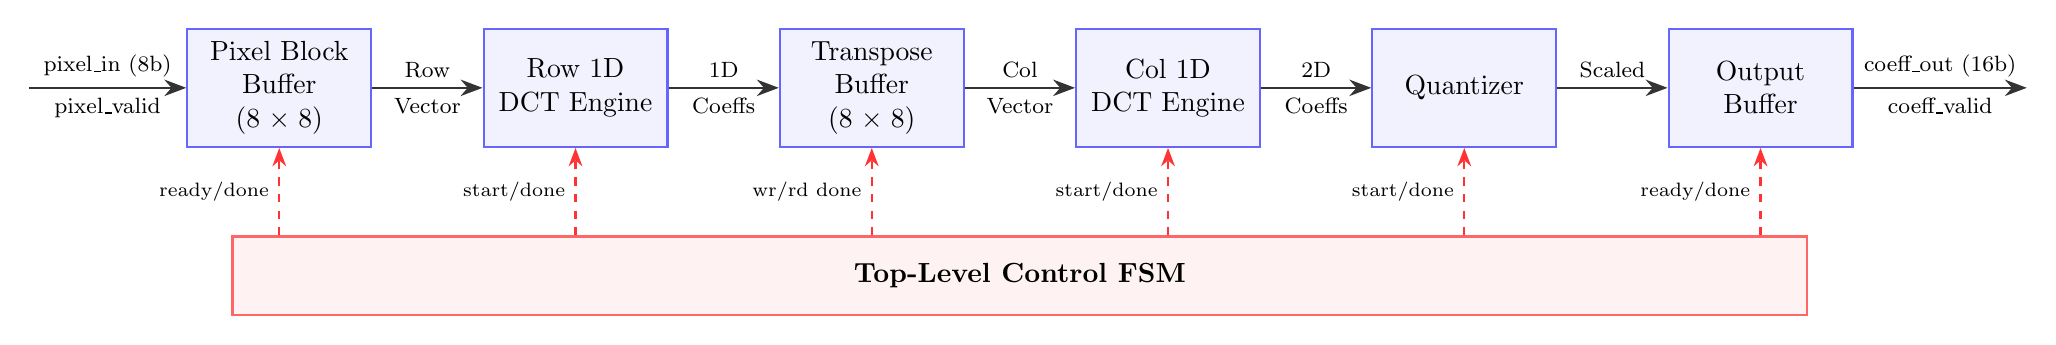
\begin{tikzpicture}[
        node distance=1.2cm and 1.4cm,
        box/.style={rectangle, draw=blue!60, fill=blue!5, thick, minimum width=2.2cm, minimum height=1.5cm, align=center, text width=2.1cm},
        fsm/.style={rectangle, draw=red!60, fill=red!5, thick, minimum width=20cm, minimum height=1cm, align=center},
        arrow/.style={-{Stealth[scale=1.2]}, thick, draw=black!80},
        dashedarrow/.style={-{Stealth[scale=1.0]}, dashed, draw=red!80, thick}
    ]

    % Nodes
    \node[box] (pbb) {Pixel Block\\Buffer\\($8\times 8$)};
    \node[box, right=of pbb] (row) {Row 1D\\DCT Engine};
    \node[box, right=of row] (tb) {Transpose\\Buffer\\($8\times 8$)};
    \node[box, right=of tb] (col) {Col 1D\\DCT Engine};
    \node[box, right=of col] (quant) {Quantizer};
    \node[box, right=of quant] (ob) {Output\\Buffer};

    % Inputs/Outputs
    \coordinate[left=2cm of pbb] (in);
    \coordinate[right=2.2cm of ob] (out);

    % FSM Node below
    \path (pbb.south) -- (ob.south) node[midway, below=1.5cm] (fsm_center) {};
    \node[fsm] at (fsm_center) (fsm) {\textbf{Top-Level Control FSM}};

    % Data path arrows
    \draw[arrow] (in) -- node[above, font=\footnotesize] {pixel\_in (8b)} node[below, font=\footnotesize] {pixel\_valid} (pbb);
    \draw[arrow] (pbb) -- node[above, font=\footnotesize] {Row} node[below, font=\footnotesize] {Vector} (row);
    \draw[arrow] (row) -- node[above, font=\footnotesize] {1D} node[below, font=\footnotesize] {Coeffs} (tb);
    \draw[arrow] (tb) -- node[above, font=\footnotesize] {Col} node[below, font=\footnotesize] {Vector} (col);
    \draw[arrow] (col) -- node[above, font=\footnotesize] {2D} node[below, font=\footnotesize] {Coeffs} (quant);
    \draw[arrow] (quant) -- node[above, font=\footnotesize] {Scaled} (ob);
    \draw[arrow] (ob) -- node[above, font=\footnotesize] {coeff\_out (16b)} node[below, font=\footnotesize] {coeff\_valid} (out);

    % Control arrows
    \draw[dashedarrow] (fsm.north -| pbb) -- node[left, font=\scriptsize] {ready/done} (pbb.south);
    \draw[dashedarrow] (fsm.north -| row) -- node[left, font=\scriptsize] {start/done} (row.south);
    \draw[dashedarrow] (fsm.north -| tb)  -- node[left, font=\scriptsize] {wr/rd done} (tb.south);
    \draw[dashedarrow] (fsm.north -| col) -- node[left, font=\scriptsize] {start/done} (col.south);
    \draw[dashedarrow] (fsm.north -| quant) -- node[left, font=\scriptsize] {start/done} (quant.south);
    \draw[dashedarrow] (fsm.north -| ob)  -- node[left, font=\scriptsize] {ready/done} (ob.south);

    \end{tikzpicture}
    }
    \caption{Top-level architectural dataflow and control hierarchy of the 2D DCT Accelerator.}
    \label{fig:system_block_diagram}
\end{figure}

\subsection{Design Space Parameterization (D1--D4)}
To thoroughly evaluate the area-throughput Pareto frontier, the RTL utilizes \texttt{generate} blocks to instantiate four unique structural variations (D1 through D4), controlled by \texttt{PIPELINED} and \texttt{PARALLEL} parameters.

\subsubsection{D1: Baseline Scalar Engine}
The D1 configuration (\texttt{PIPELINED=0}, \texttt{PARALLEL=0}) represents the minimal area footprint. The 1D engine contains a single Multiply-Accumulate (MAC) unit. It processes one pixel per clock cycle, requiring 64 cycles to complete a 1D transform of an $8 \times 8$ block (512 cycles total for the full 2D DCT). Figure \ref{fig:rtl_d1} illustrates the synthesized baseline hierarchy.

\begin{figure}[H]
    \centering
    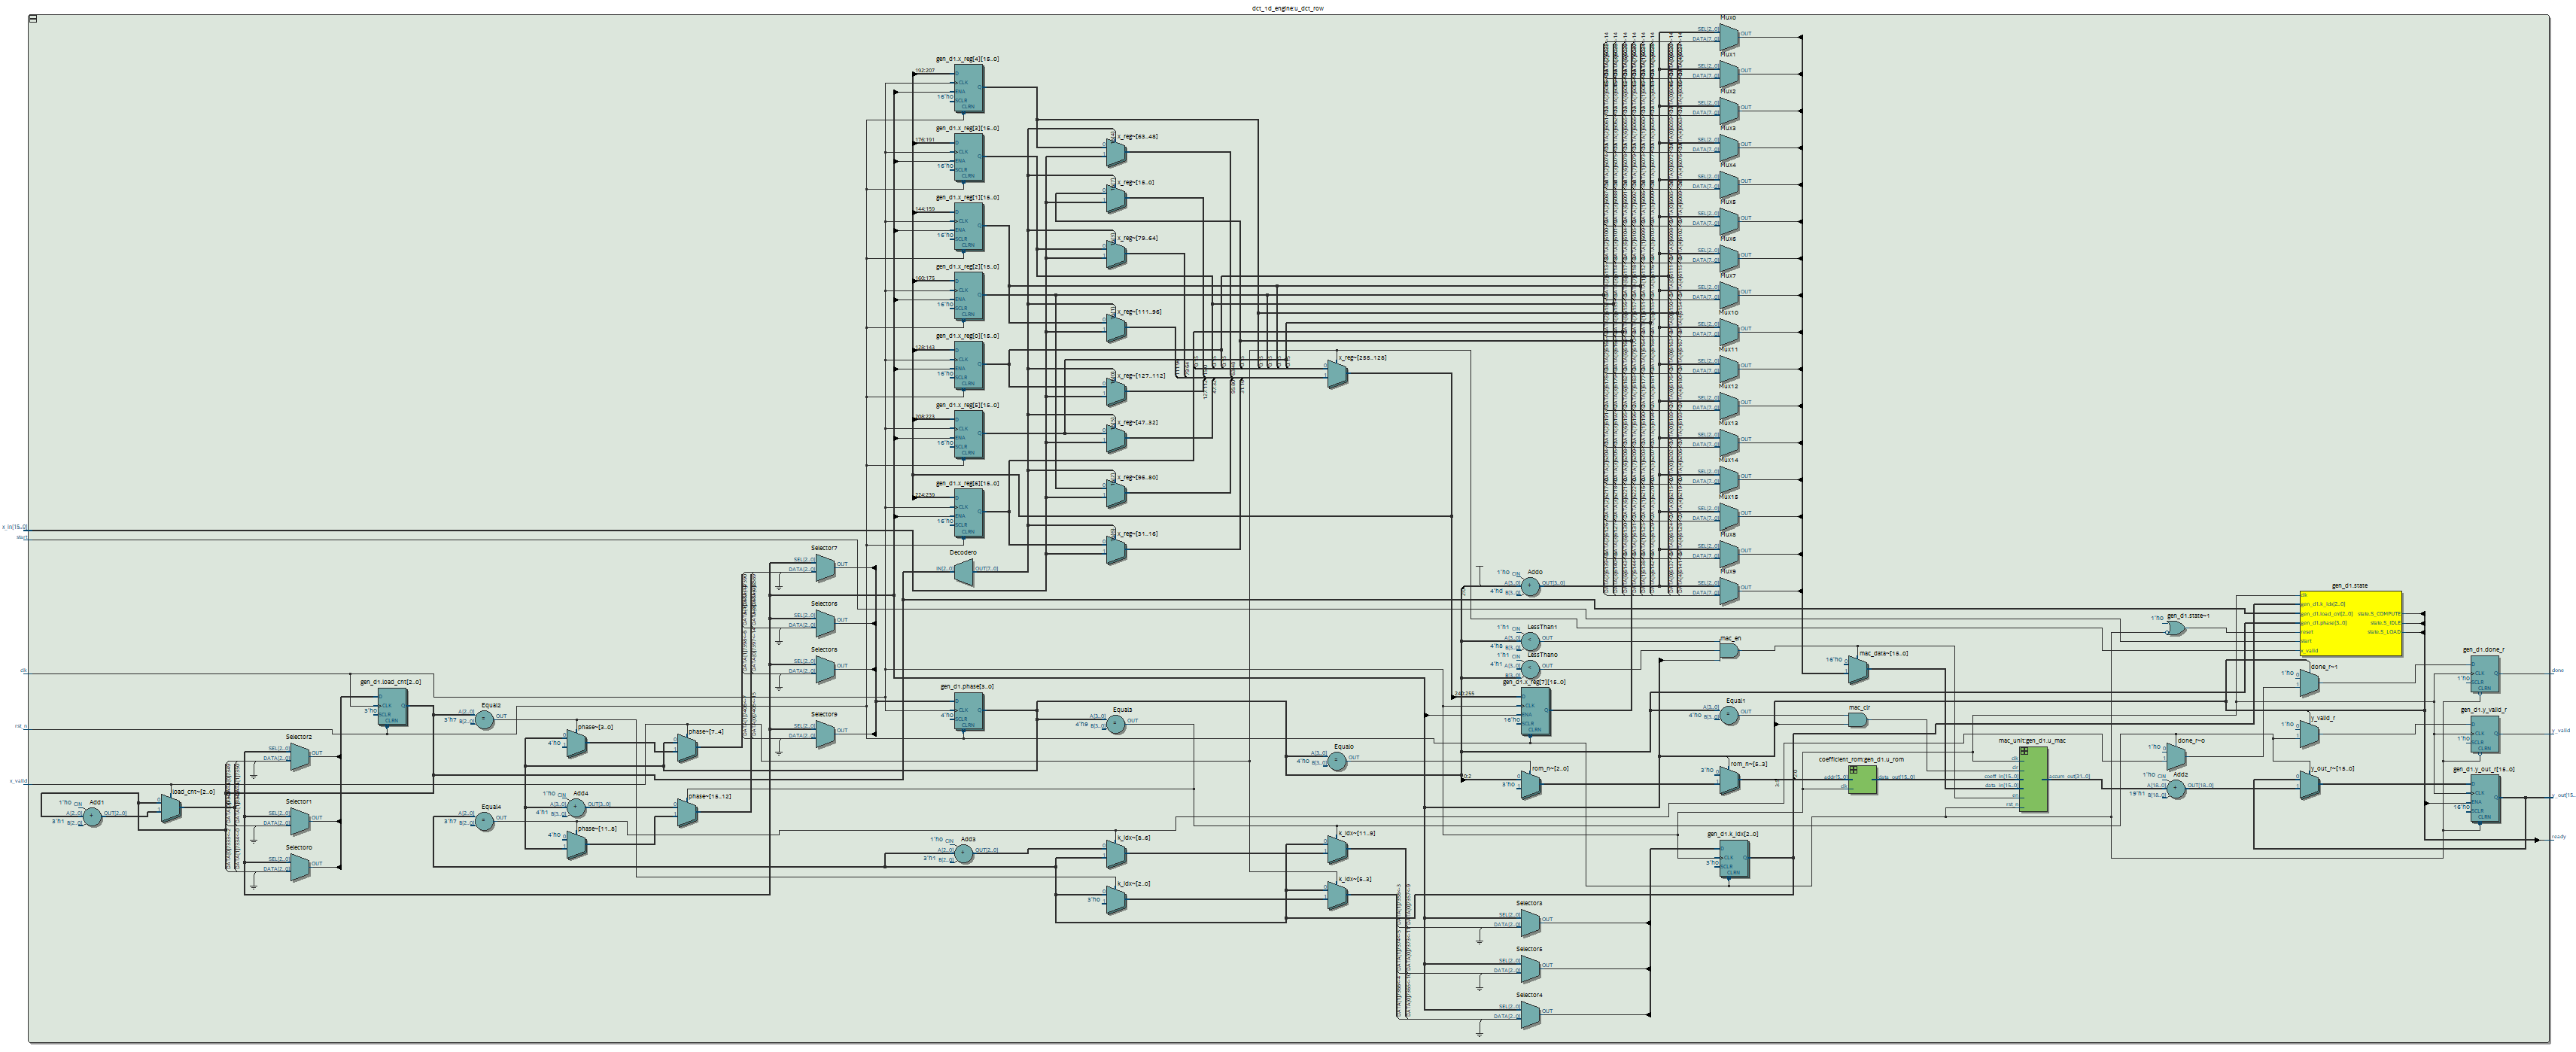
\includegraphics[width=\textwidth]{rtl_viewer_D1.png}
    \caption{RTL Viewer Schematic for D1 (Baseline) architecture. This minimal design instantiates a single shared Multiply-Accumulate (MAC) unit and a finite state machine that sequentially feeds pixel and coefficient data through the datapath, prioritizing absolute minimal area footprint at the cost of high latency.}
    \label{fig:rtl_d1}
\end{figure}

\subsubsection{D2: Pipelined Scalar Engine}
The D2 configuration (\texttt{PIPELINED=1}, \texttt{PARALLEL=0}) maintains the single MAC unit but introduces deep pipeline registers between the multiplier and accumulator stages, as well as intermediate buffer registers. While the cycle latency remains 512 cycles, the critical path is drastically shortened, allowing the maximum clock frequency ($F_{max}$) to double compared to D1.

\begin{figure}[H]
    \centering
    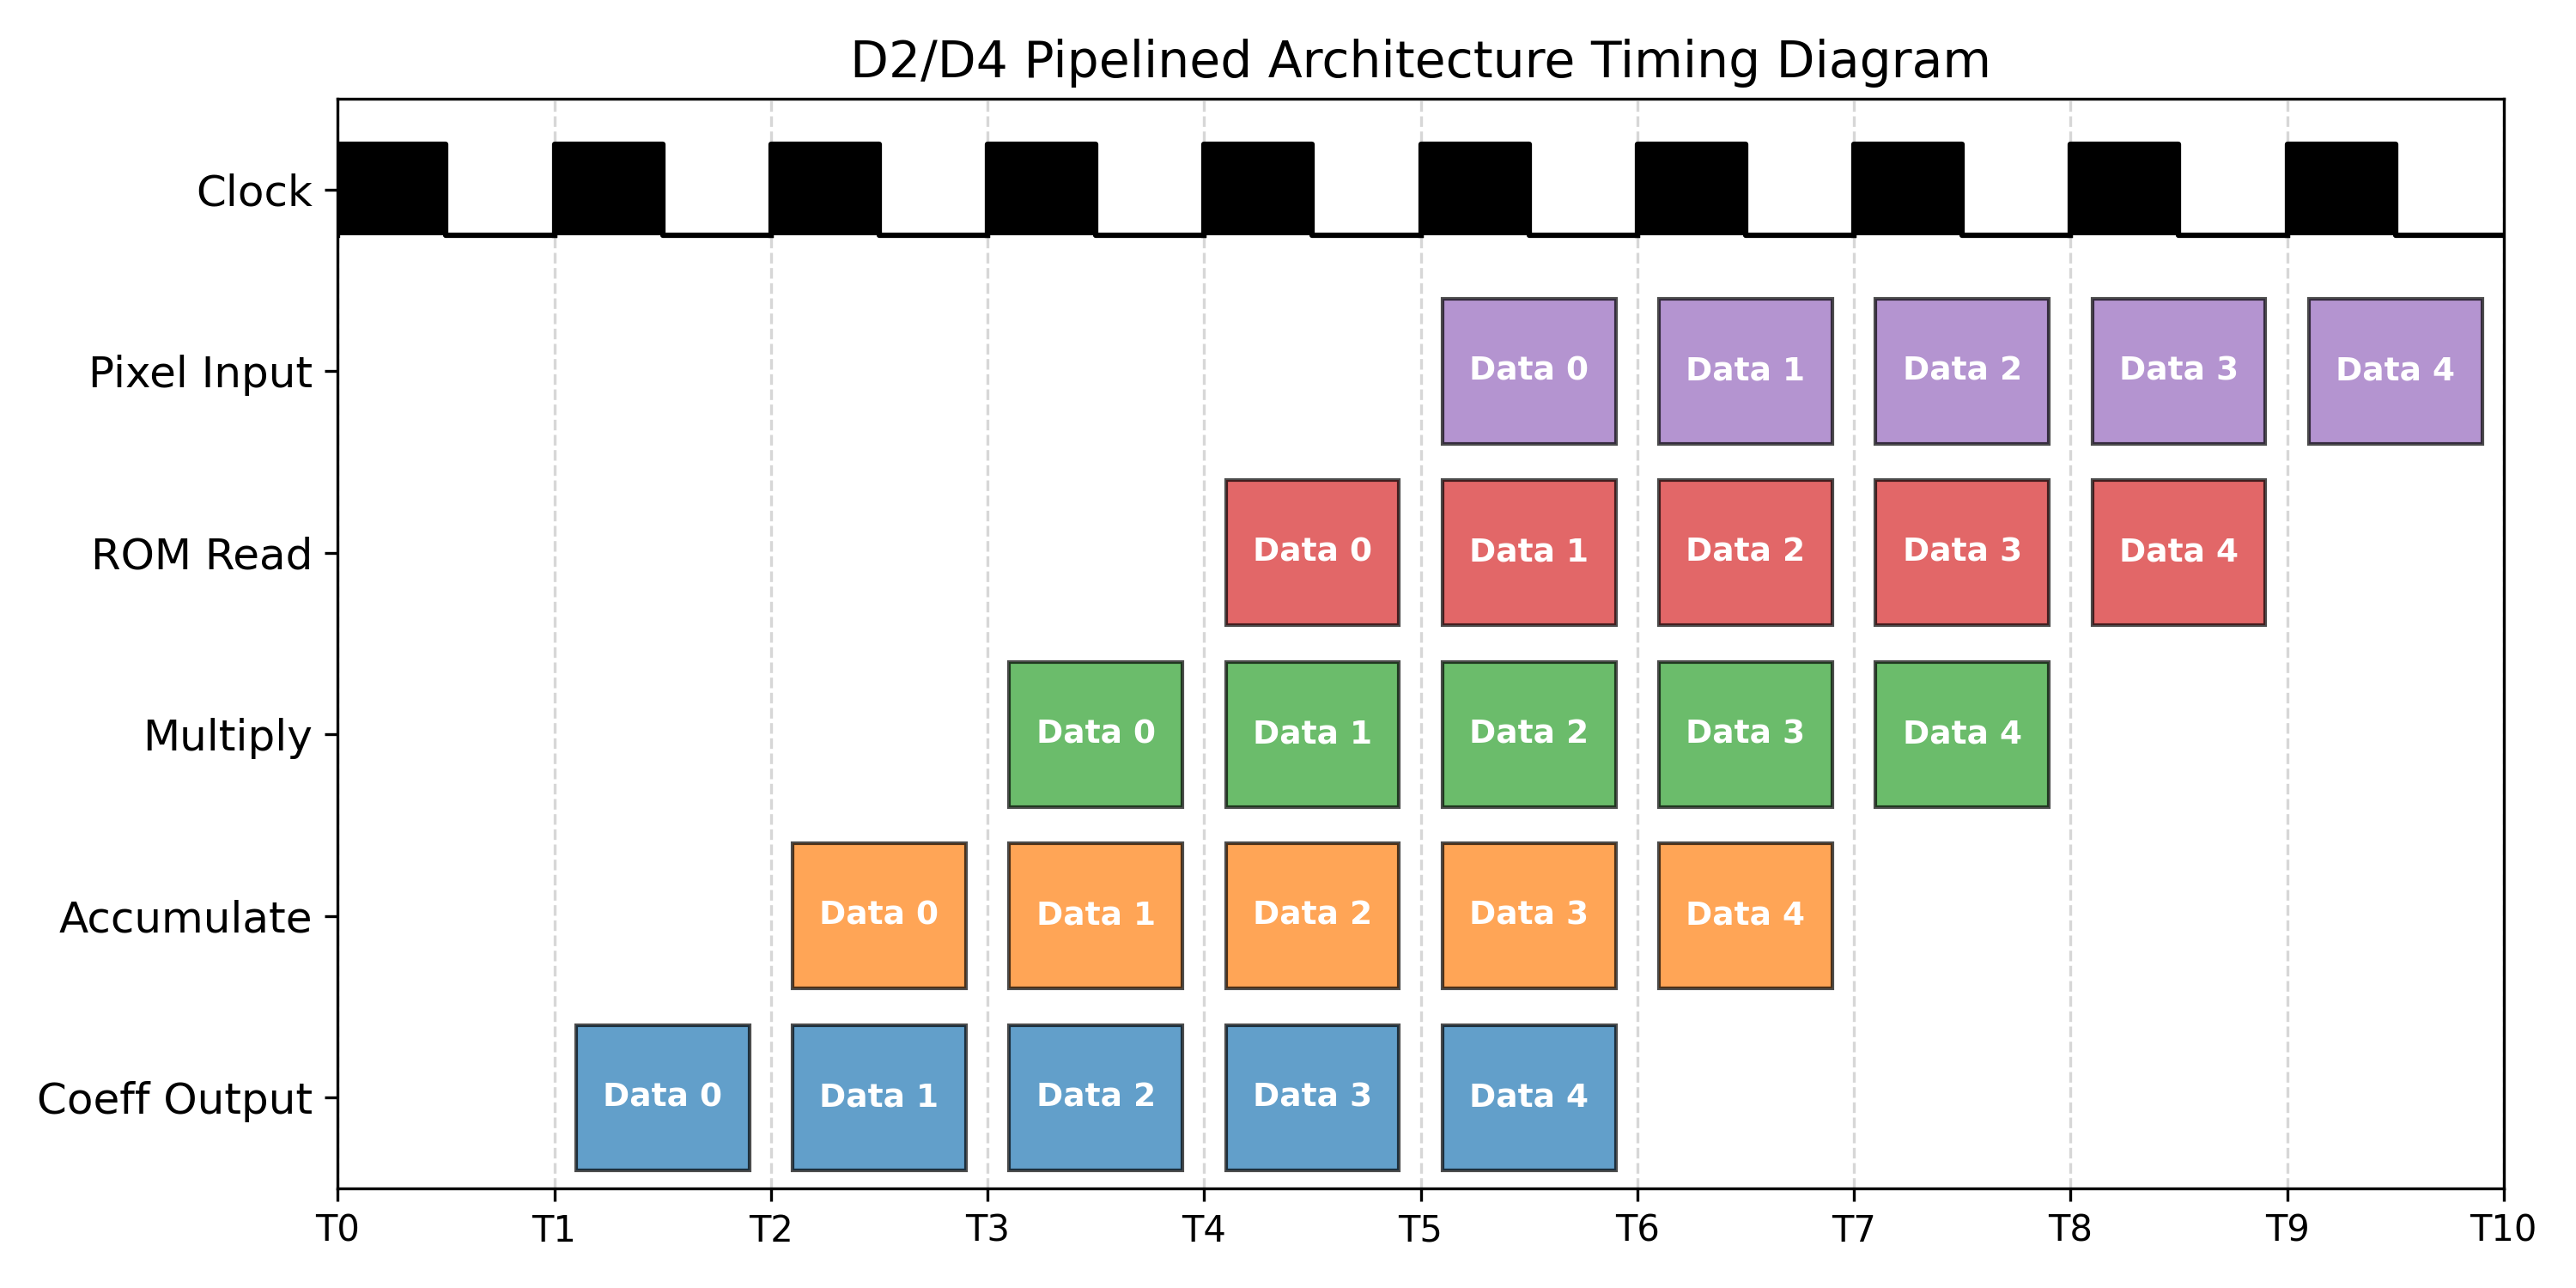
\includegraphics[width=\textwidth]{pipeline_waveform.png}
    \caption{Pipeline timing diagram illustrating data flow and stage progression across the D2 architecture. Notice how the valid signals propagate sequentially through the multiplier, adder, and accumulator stages, ensuring high-frequency operation without combinational logic bottlenecks.}
    \label{fig:pipeline_waveform}
\end{figure}

\begin{figure}[H]
    \centering
    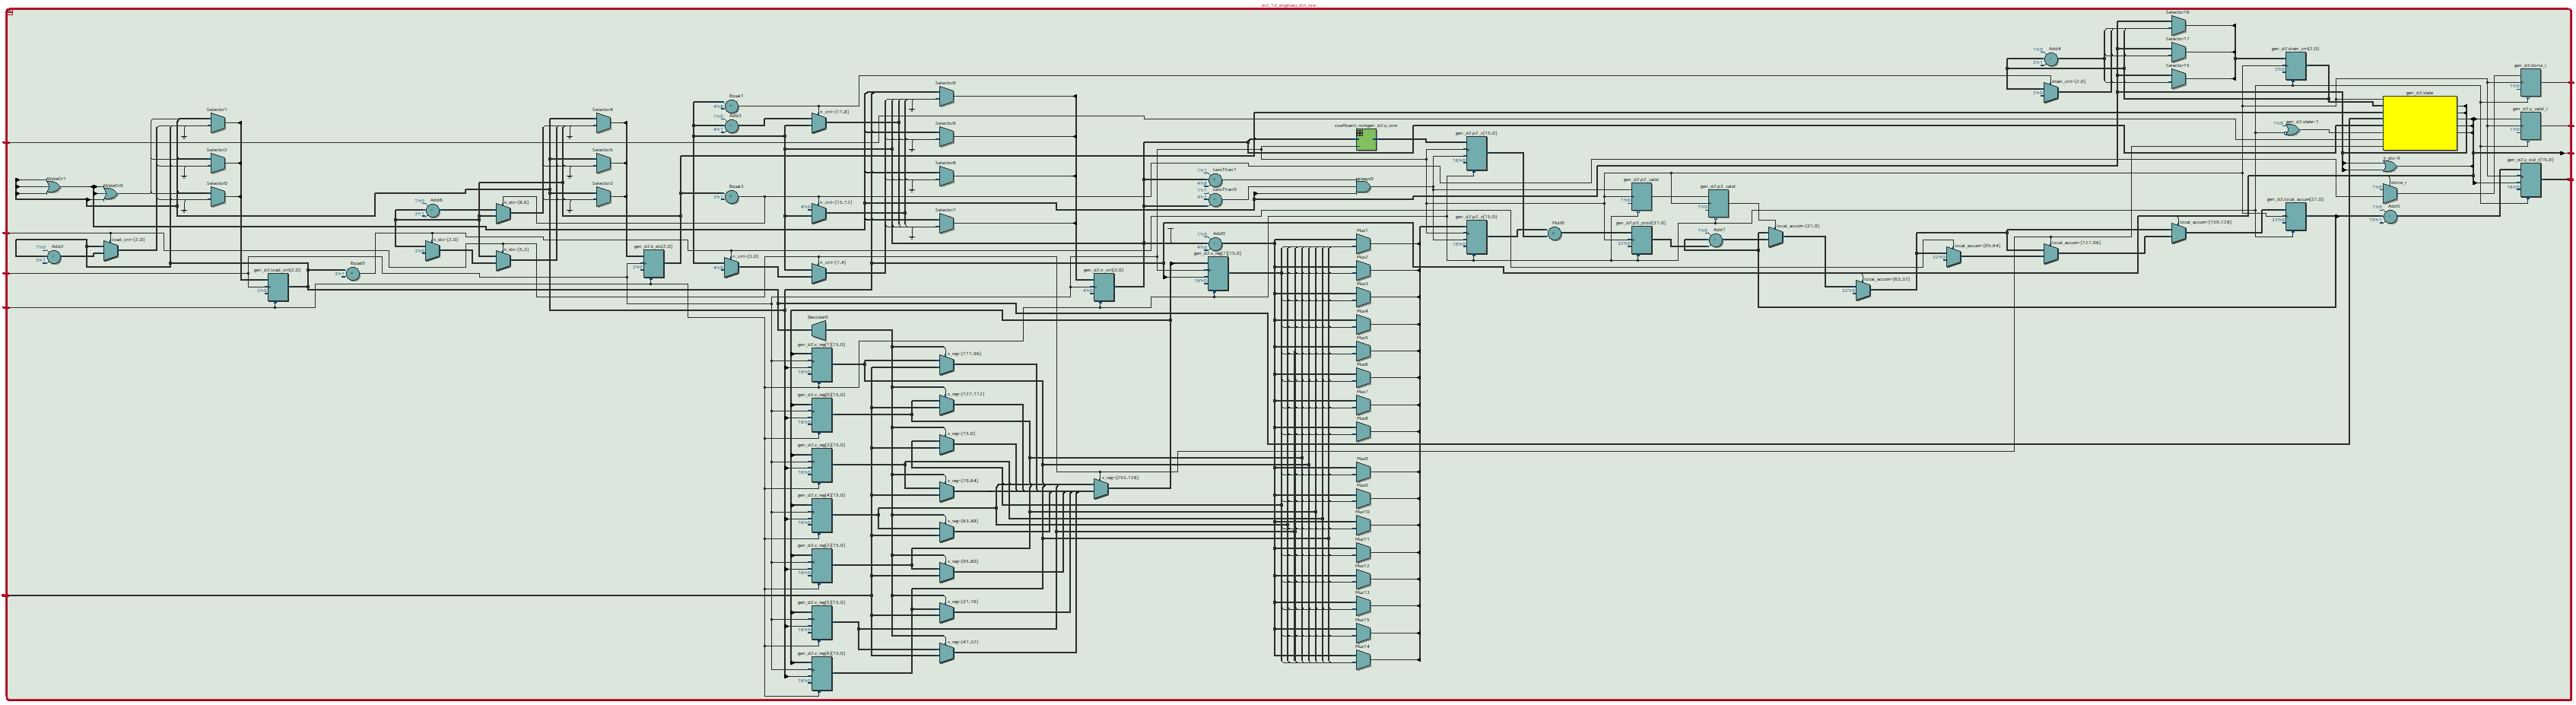
\includegraphics[width=\textwidth]{rtl_viewer_D2.png}
    \caption{RTL Viewer Schematic for D2 (Pipelined) architecture. The addition of dedicated pipeline registers (visible separating the arithmetic multiplier and adder stages) breaks the critical path of the single MAC unit, allowing for a significantly higher maximum clock frequency.}
    \label{fig:rtl_d2}
\end{figure}

\subsubsection{D3: Parallel Array Engine}
The D3 configuration (\texttt{PIPELINED=0}, \texttt{PARALLEL=1}) optimizes for cycle latency by instantiating an 8-way parallel MAC array within the 1D engine. This allows an entire row or column to be multiplied by the basis coefficients simultaneously. The latency is reduced to 8 cycles for a 1D transform, yielding a total 2D latency of just 64 cycles.

\begin{figure}[H]
    \centering
    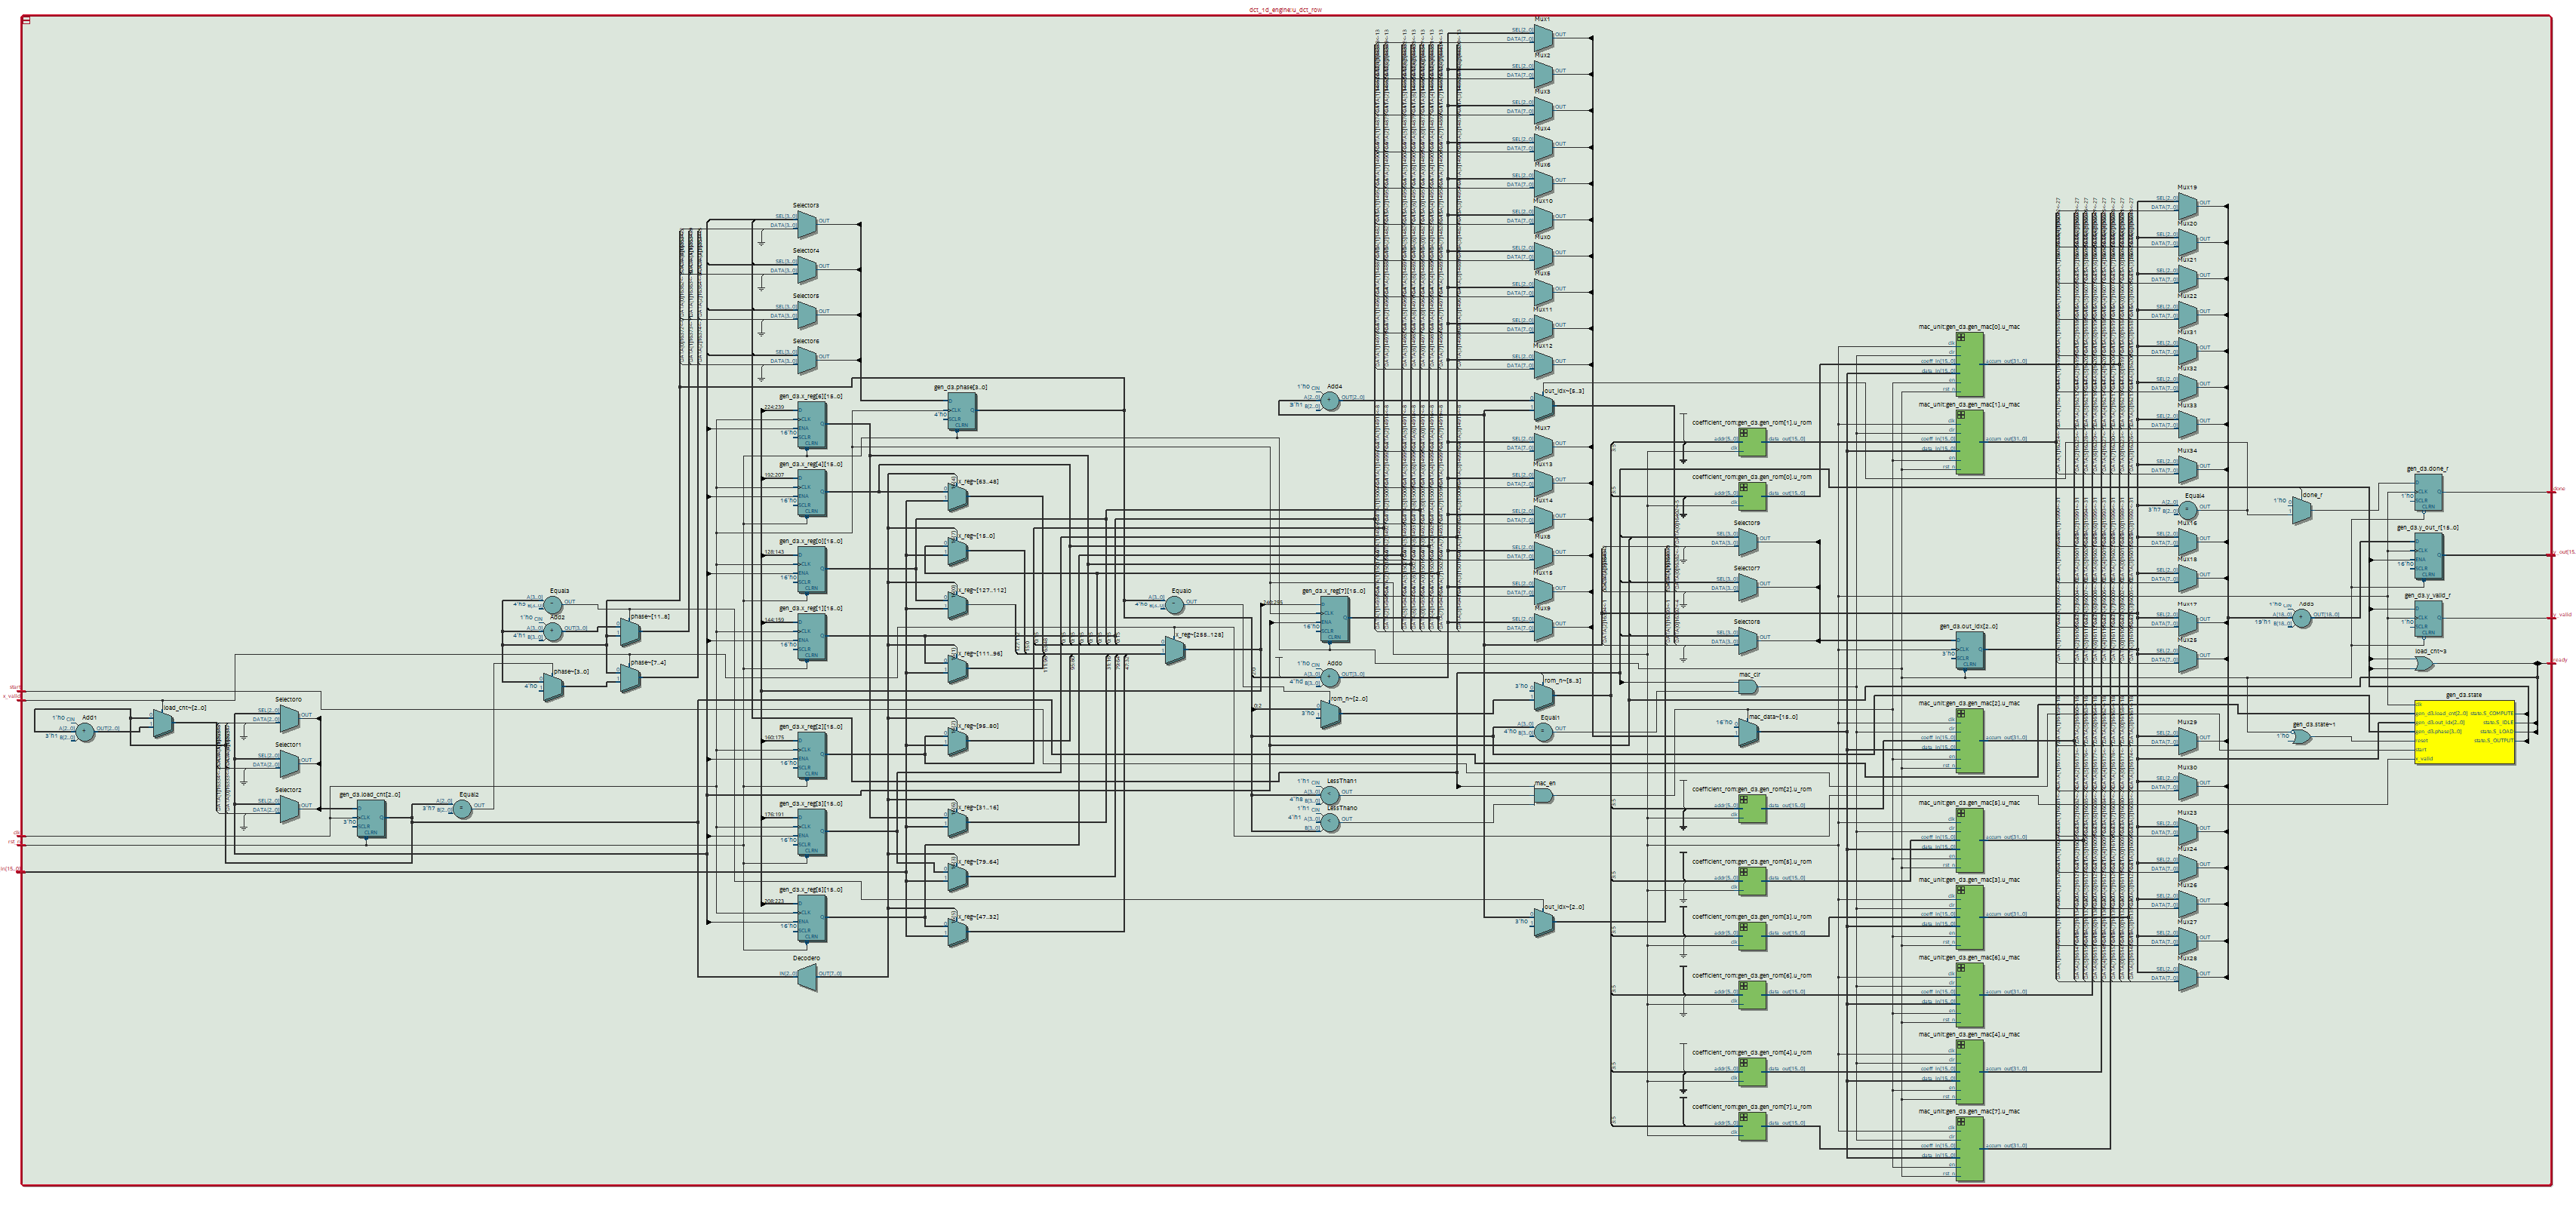
\includegraphics[width=\textwidth]{rtl_viewer_D3.png}
    \caption{RTL Viewer Schematic for D3 (Parallel) architecture. Notice the eight parallel MAC units instantiated across the datapath. This broadcast architecture allows an entire column of 8 basis coefficients to be multiplied and accumulated simultaneously against a single pixel.}
    \label{fig:rtl_d3}
\end{figure}

\begin{figure}[H]
    \centering
    \resizebox{0.9\textwidth}{!}{
    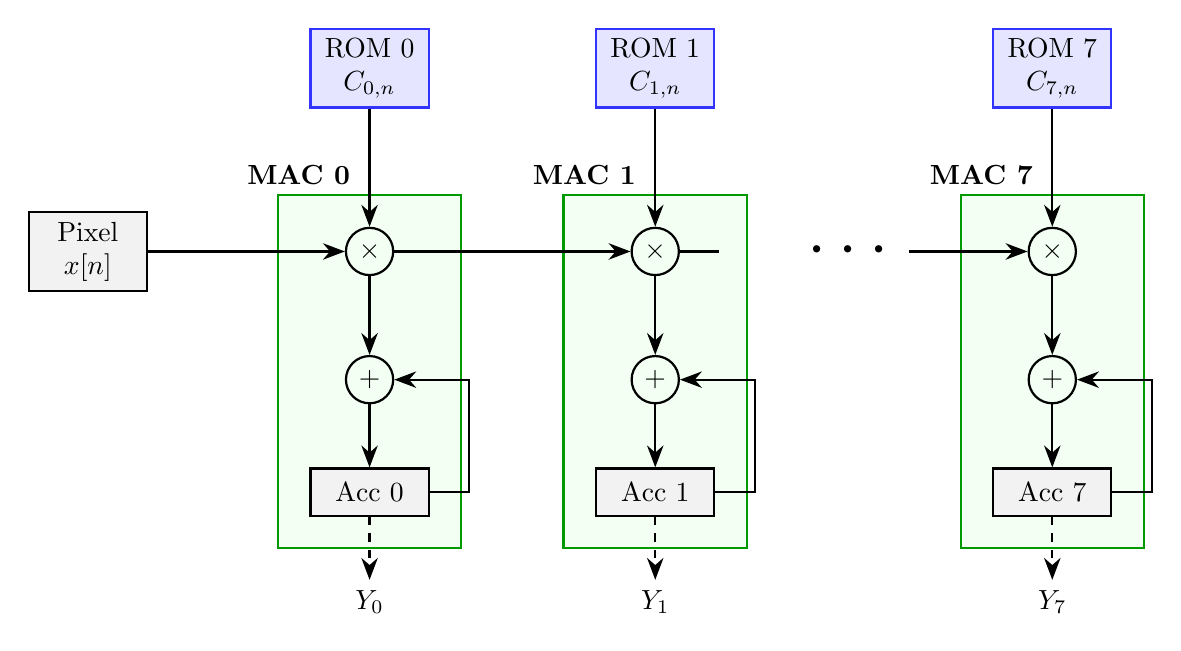
\begin{tikzpicture}[
        node distance=1.2cm and 1.5cm,
        register/.style={rectangle, draw=black, fill=gray!10, thick, minimum width=1.5cm, minimum height=1cm, align=center},
        rom/.style={rectangle, draw=blue!80, fill=blue!10, thick, minimum width=1.5cm, minimum height=1cm, align=center},
        mac/.style={rectangle, draw=green!60!black, fill=green!5, thick, inner sep=0.4cm},
        adder/.style={circle, draw=black, thick, minimum size=0.6cm, inner sep=0pt},
        mult/.style={circle, draw=black, thick, minimum size=0.6cm, inner sep=0pt},
        arrow/.style={-{Stealth[scale=1.2]}, thick},
        dots/.style={font=\Huge, align=center}
    ]

    % Multipliers define the horizontal center line
    \node[mult] (m0) {$\times$};
    \node[mult, right=3cm of m0] (m1) {$\times$};
    \node[dots, right=1.5cm of m1] (dots) {$\cdots$};
    \node[mult, right=1.5cm of dots] (m7) {$\times$};

    % Input Register on the left
    \node[register, left=2.5cm of m0] (xreg) {Pixel\\$x[n]$};

    % ROMs above multipliers
    \node[rom, above=1.5cm of m0] (rom0) {ROM 0\\$C_{0,n}$};
    \node[rom, above=1.5cm of m1] (rom1) {ROM 1\\$C_{1,n}$};
    \node[rom, above=1.5cm of m7] (rom7) {ROM 7\\$C_{7,n}$};

    % Adders below multipliers
    \node[adder, below=1cm of m0] (a0) {$+$};
    \node[adder, below=1cm of m1] (a1) {$+$};
    \node[adder, below=1cm of m7] (a7) {$+$};

    % Accumulators below adders
    \node[register, minimum height=0.6cm, below=0.8cm of a0] (acc0) {Acc 0};
    \node[register, minimum height=0.6cm, below=0.8cm of a1] (acc1) {Acc 1};
    \node[register, minimum height=0.6cm, below=0.8cm of a7] (acc7) {Acc 7};

    % Draw MAC unit bounding boxes using fit on background layer
    \begin{scope}[on background layer]
        \node[mac, fit=(m0) (a0) (acc0), label={[font=\bfseries, xshift=-0.9cm]above:MAC 0}] (mac0) {};
        \node[mac, fit=(m1) (a1) (acc1), label={[font=\bfseries, xshift=-0.9cm]above:MAC 1}] (mac1) {};
        \node[mac, fit=(m7) (a7) (acc7), label={[font=\bfseries, xshift=-0.9cm]above:MAC 7}] (mac7) {};
    \end{scope}

    % Broadcast x[n]
    \draw[arrow] (xreg.east) -- (m0.west);
    \draw[arrow] (m0.east) -- (m1.west);
    \draw[thick] (m1.east) -- +(0.5,0);
    \draw[arrow] (dots.east) -- (m7.west);

    % ROM to Mult
    \draw[arrow] (rom0.south) -- (m0.north);
    \draw[arrow] (rom1.south) -- (m1.north);
    \draw[arrow] (rom7.south) -- (m7.north);

    % Mult to Adder
    \draw[arrow] (m0.south) -- (a0.north);
    \draw[arrow] (m1.south) -- (a1.north);
    \draw[arrow] (m7.south) -- (a7.north);

    % Adder to Acc
    \draw[arrow] (a0.south) -- (acc0.north);
    \draw[arrow] (a1.south) -- (acc1.north);
    \draw[arrow] (a7.south) -- (acc7.north);

    % Acc Feedback to Adder
    \draw[arrow] (acc0.east) -- +(0.5,0) |- (a0.east);
    \draw[arrow] (acc1.east) -- +(0.5,0) |- (a1.east);
    \draw[arrow] (acc7.east) -- +(0.5,0) |- (a7.east);

    % Outputs
    \draw[arrow, dashed] (acc0.south) -- +(0,-0.8) node[below] {$Y_0$};
    \draw[arrow, dashed] (acc1.south) -- +(0,-0.8) node[below] {$Y_1$};
    \draw[arrow, dashed] (acc7.south) -- +(0,-0.8) node[below] {$Y_7$};

    \end{tikzpicture}
    }
    \caption{D3 Parallel Array Engine datapath: A single pixel $x[n]$ is broadcast to 8 parallel MAC units, each simultaneously multiplying it by a unique basis coefficient $C_{k,n}$.}
    \label{fig:mac_schematic}
\end{figure}

\subsubsection{D4: Pipelined and Parallel Engine}
The D4 configuration (\texttt{PIPELINED=1}, \texttt{PARALLEL=1}) is the most aggressive architecture. It combines the 8-way parallel MAC array to process 8 pixels per cycle, while inserting pipeline registers to break the critical paths generated by the wide parallel adders. This results in the highest absolute throughput (Blocks/sec), achieving a latency of 64 cycles while operating at nearly 200 MHz.

\begin{figure}[H]
    \centering
    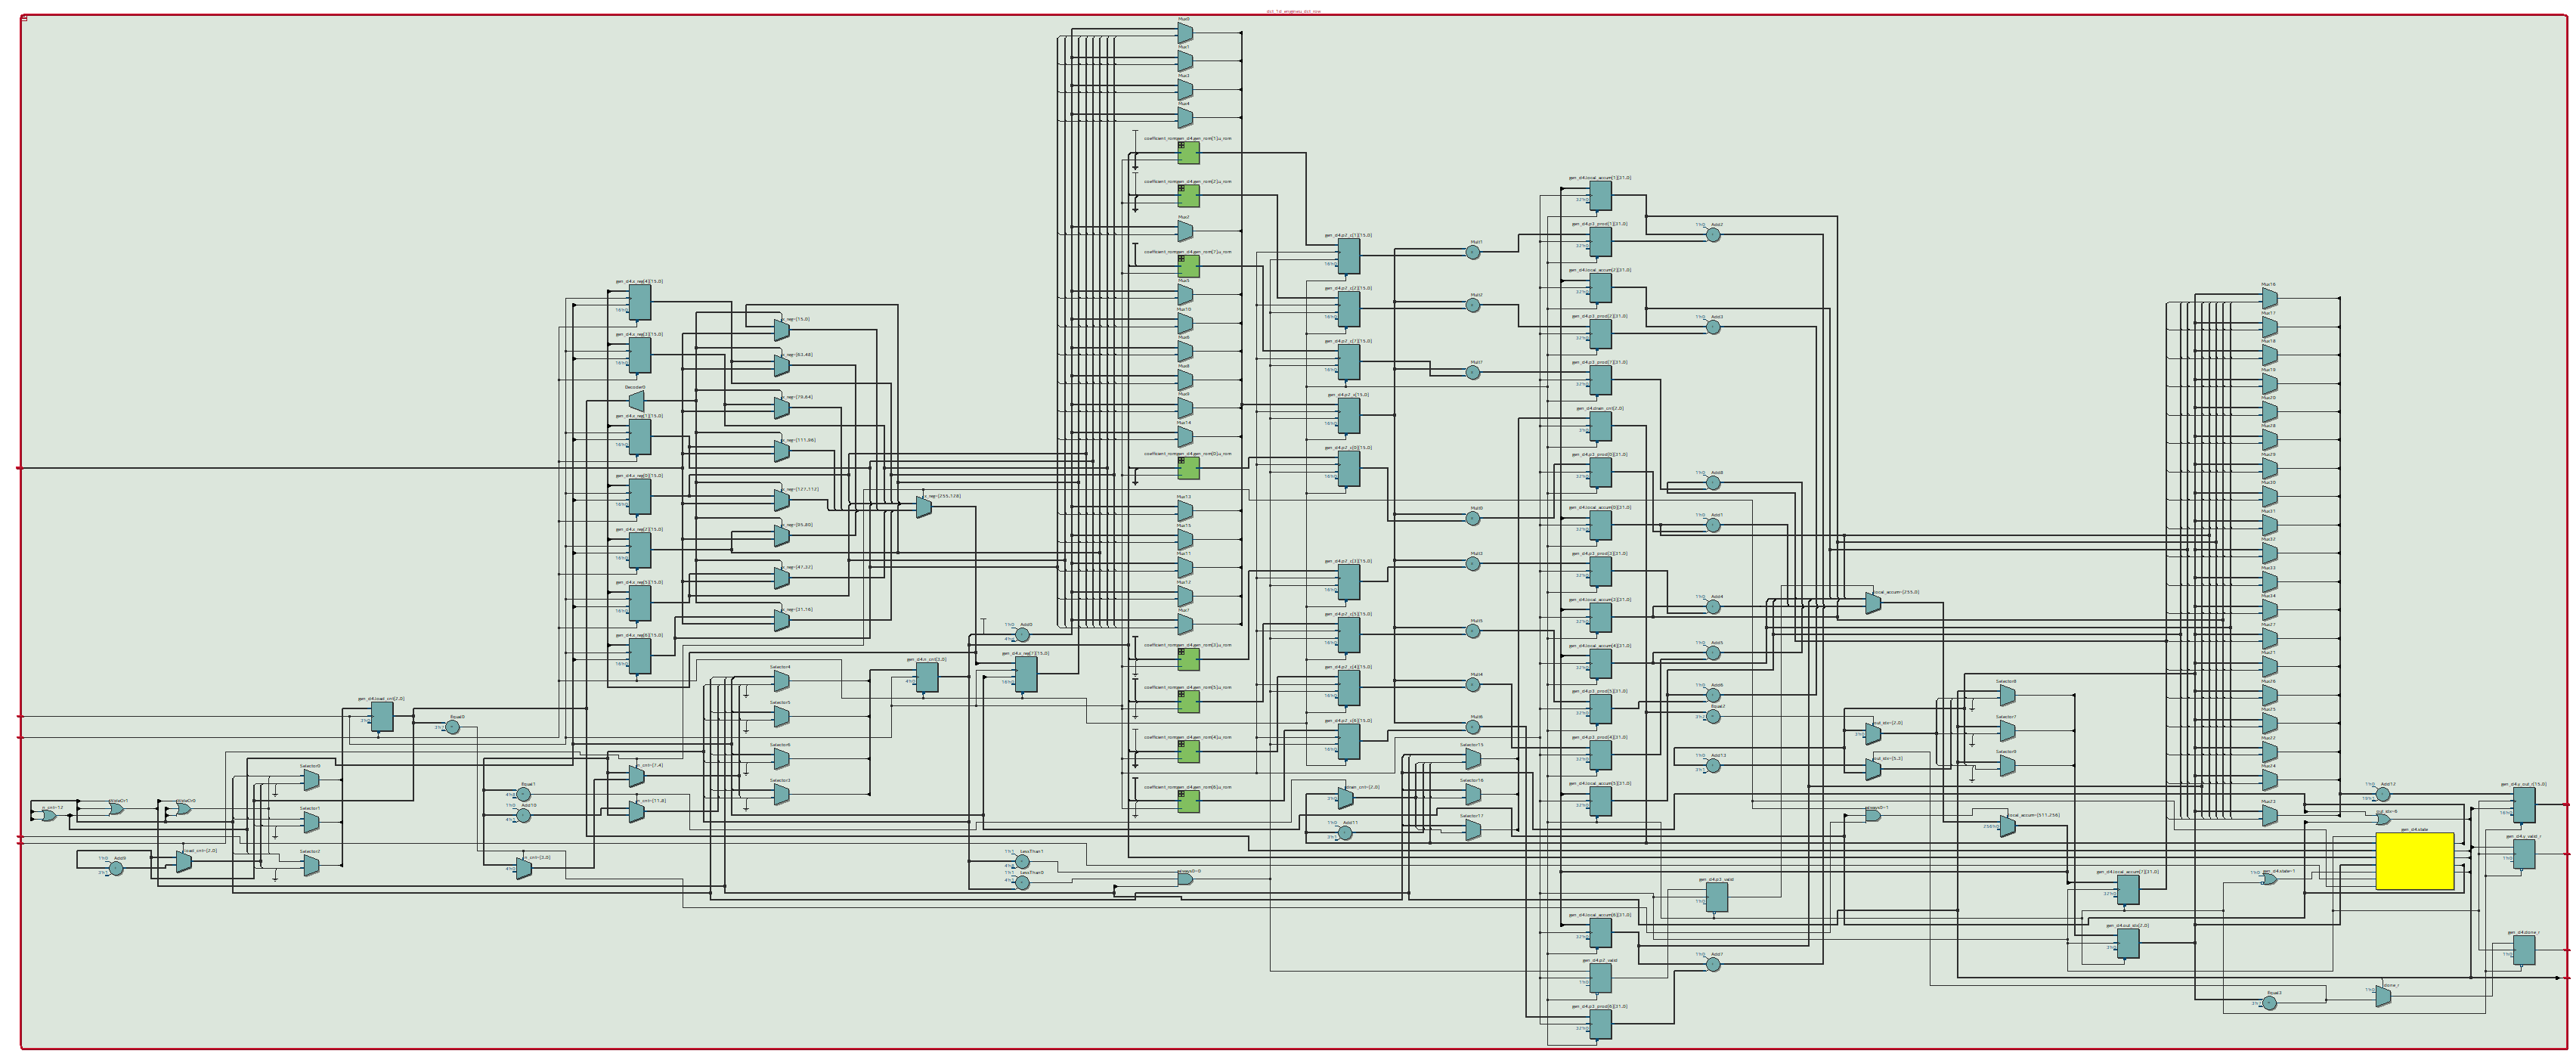
\includegraphics[width=\textwidth]{rtl_viewer_D4.png}
    \caption{RTL Viewer Schematic for D4 (Pipelined + Parallel) architecture. This configuration orthogonally combines the 8-way spatial parallelism of D3 with the deep register pipelining of D2, representing the highest performance tier and optimal throughput-to-area design point.}
    \label{fig:rtl_d4}
\end{figure}

\section{Verification}

Ensuring the functional correctness of the hardware across all four architectural configurations requires a robust, automated verification pipeline. The methodology relies on comparing the SystemVerilog RTL simulation outputs against a software-generated golden reference.

\subsection{Golden Reference Generation}
To establish a ground truth, a high-level mathematical model of the 2D DCT was developed using MATLAB and Python. This software model applies the exact 16-bit Q2.14 fixed-point quantization scheme used in the hardware datapath. By simulating the precision loss in software, the generated output coefficients serve as a bit-accurate ``golden reference.'' The Python infrastructure processes standard test images, extracts $8 \times 8$ pixel blocks, and exports both the raw input pixels and the expected output coefficients to flat text files for the RTL testbench to ingest.

\subsection{Testbench Methodology}
The SystemVerilog testbench is designed to be highly automated and parameter-aware. Using standard file I/O operations (\texttt{\$readmemh} and \texttt{\$fopen}), the testbench streams the raw pixel data into the \texttt{top\_dct\_accelerator} module while strictly adhering to the valid/ready handshake protocol of the hardware interface. 

As the accelerator processes the blocks, the testbench captures the 2D frequency coefficients and performs a real-time comparison against the golden reference data. Because the hardware datapath performs multiple stages of fixed-point truncation and rounding, minor least-significant bit (LSB) deviations from the ideal Python mathematical model are expected. Therefore, the testbench implements a $\pm 2$ LSB tolerance threshold. If all hardware outputs fall within this strict error margin, the specific design point (D1--D4) is verified as functionally correct.

\subsection{Waveform Analysis}
In addition to automated data checking, ModelSim was utilized to perform manual waveform analysis. This was critical for debugging the intricate timing of the row-column decomposition, particularly verifying that the transposition buffer correctly filled and drained without dropping data or overwriting active rows. The waveform analysis confirmed that the pipeline stages remained fully saturated during continuous data streaming, and that the stall logic correctly handled back-pressure without corrupting the datapath state.

\begin{figure}[H]
    \centering
    \begin{subfigure}[b]{\textwidth}
        \centering
        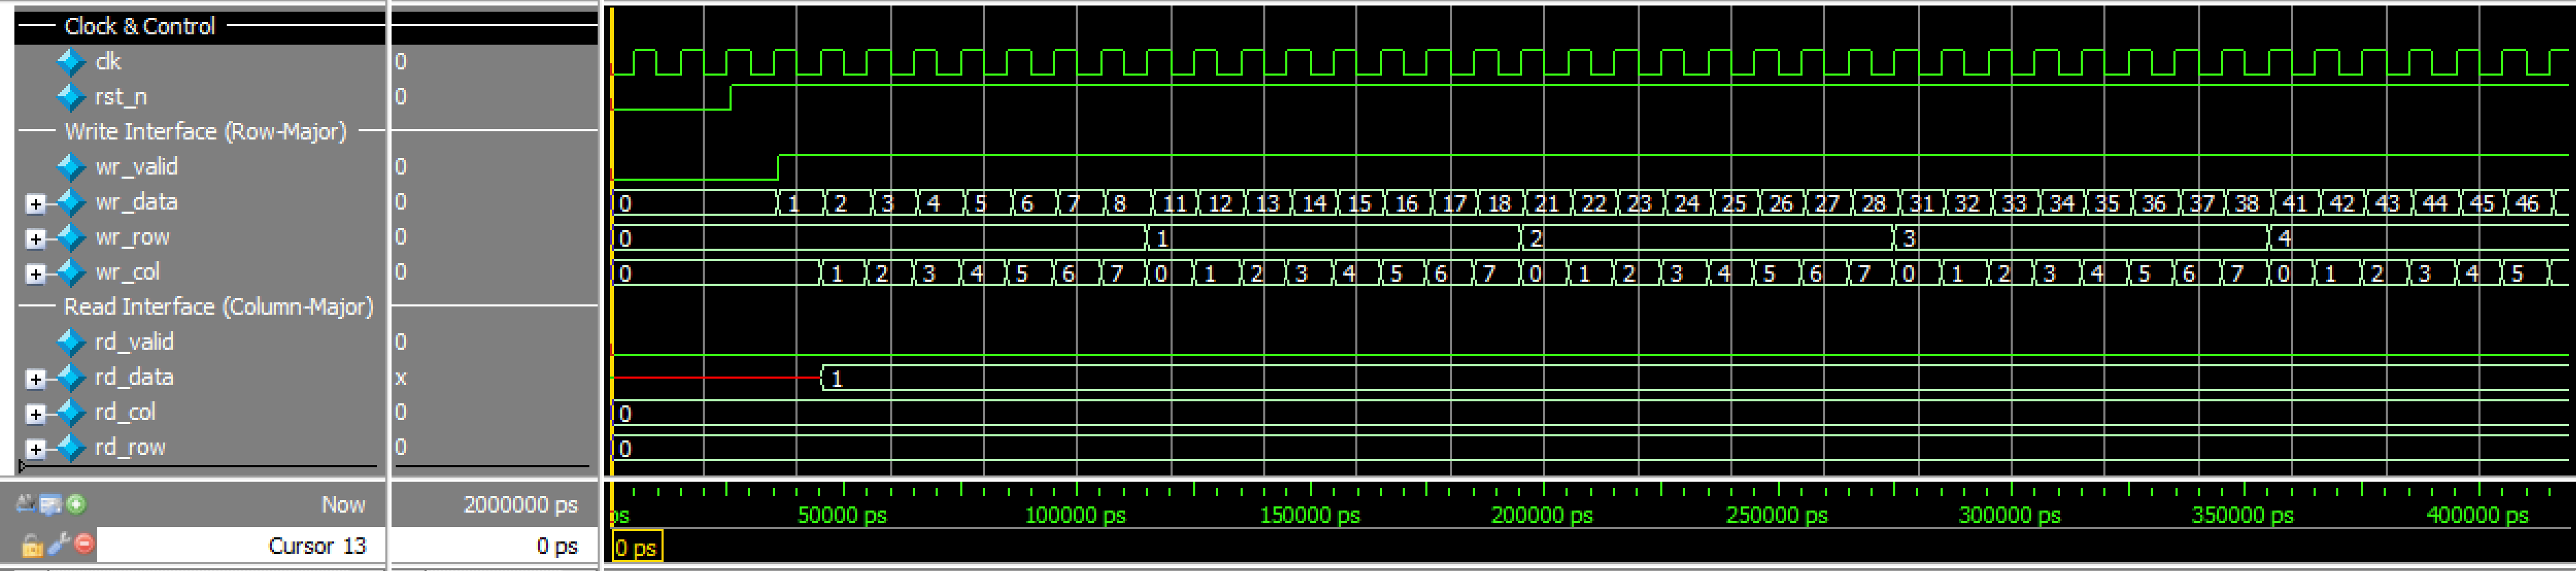
\includegraphics[width=\textwidth]{transpose_write.png}
        \caption{Write Phase (Row-Major)}
        \label{fig:transpose_write}
    \end{subfigure}

    \vspace{0.5cm}

    \begin{subfigure}[b]{\textwidth}
        \centering
        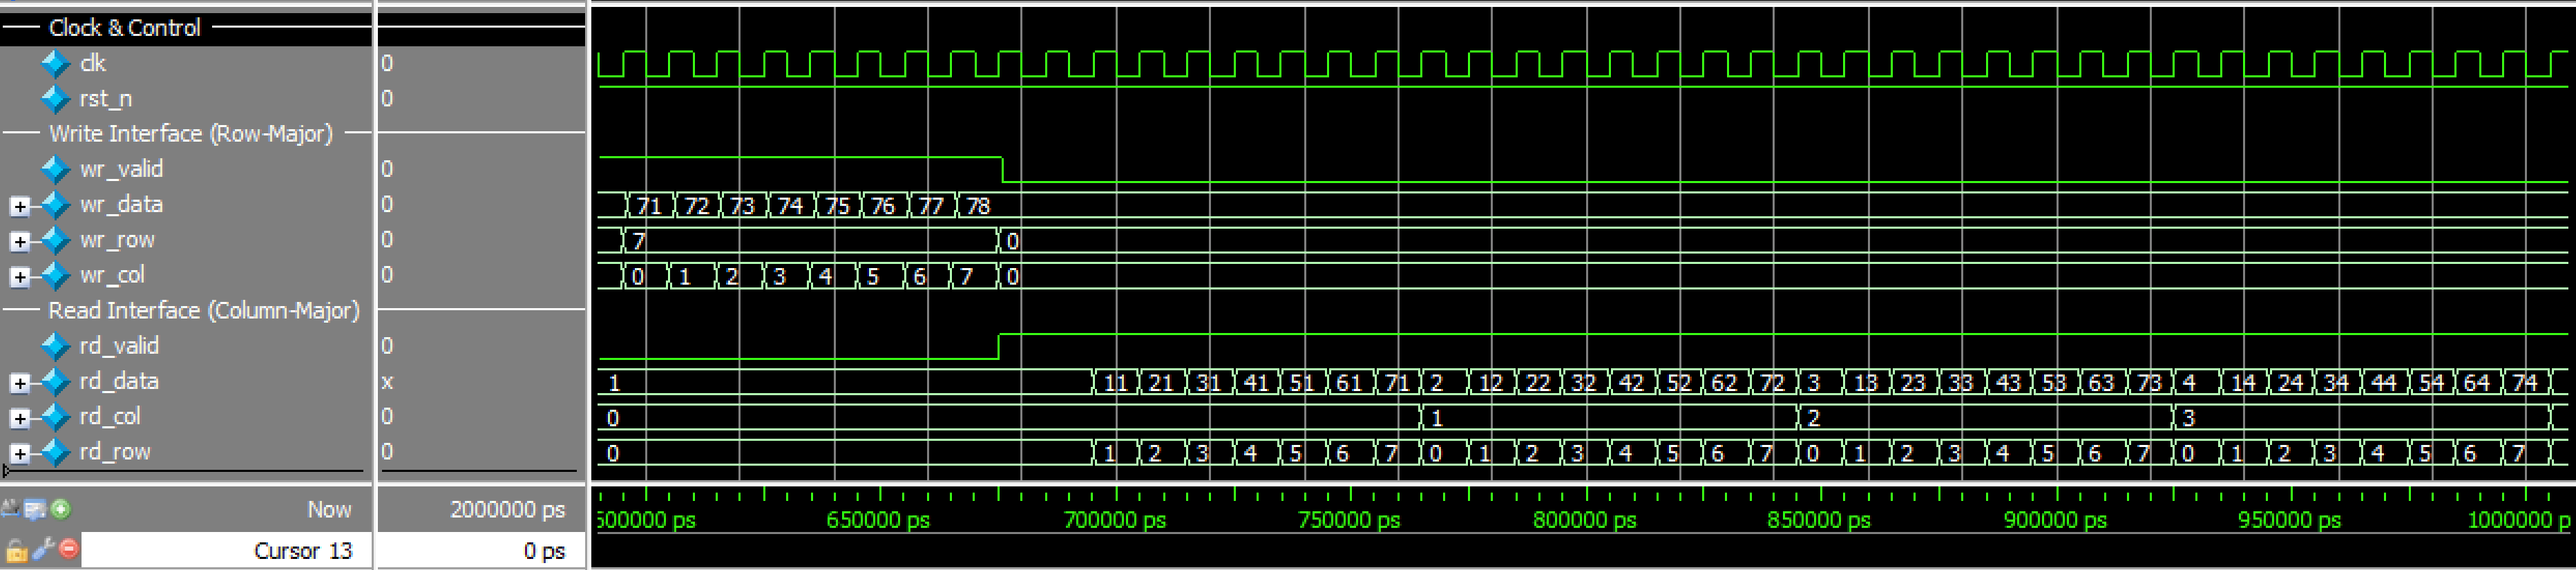
\includegraphics[width=\textwidth]{transpose_read.png}
        \caption{Read Phase (Column-Major)}
        \label{fig:transpose_read}
    \end{subfigure}
    \caption{ModelSim waveforms demonstrating the memory addressing patterns of the Transpose Buffer. During the write phase, \texttt{wr\_col} iterates rapidly (0-7) across columns while \texttt{wr\_row} increments row-by-row. During the read phase, the pattern is inverted: \texttt{rd\_row} iterates rapidly across rows while \texttt{rd\_col} increments column-by-column, successfully proving the corner-turning logic.}
    \label{fig:transpose_waveform}
\end{figure}

\section{Results}
This section analyzes the empirical performance, resource utilization, and computational fidelity of the four hardware design variations (D1--D4). All designs were synthesized targeting an Intel Cyclone V FPGA.

\subsection{Image Fidelity}
The primary objective of the 16-bit fixed-point datapath is to maintain visual quality without requiring expensive floating-point resources. As shown in Figure \ref{fig:image_comparison}, the standard Baboon test image is successfully reconstructed by the hardware accelerator with no visually perceptible degradation compared to the original image. Figure \ref{fig:image_comparison} also provides a full-range error demonstration to showcase the absolute magnitude of the reconstruction error, alongside a spatially-rescaled error plot highlighting exactly where within the image the quantization noise occurs.

Quantitatively, the architecture achieves a high Peak Signal-to-Noise Ratio (PSNR) of $51.05\text{ dB}$ and a Structural Similarity Index (SSIM) of $0.9995$ across all variants. Figure \ref{fig:psnr_vs_qf} demonstrates that this fidelity remains highly stable across various JPEG quantization factors. Additionally, Figure \ref{fig:error_histogram} illustrates the statistical distribution of numerical errors, confirming that fixed-point quantization noise is tightly bounded. While the vast majority of pixel errors fall within a strict $\pm 2$ LSB margin, a single statistical outlier with a difference of $+3$ LSB is present. This is entirely mathematically expected; it represents the worst-case compound accumulation of fractional truncation across the two separable 1D transformation passes when compared against an ideal double-precision floating-point reference.

\begin{figure}[H]
    \centering
    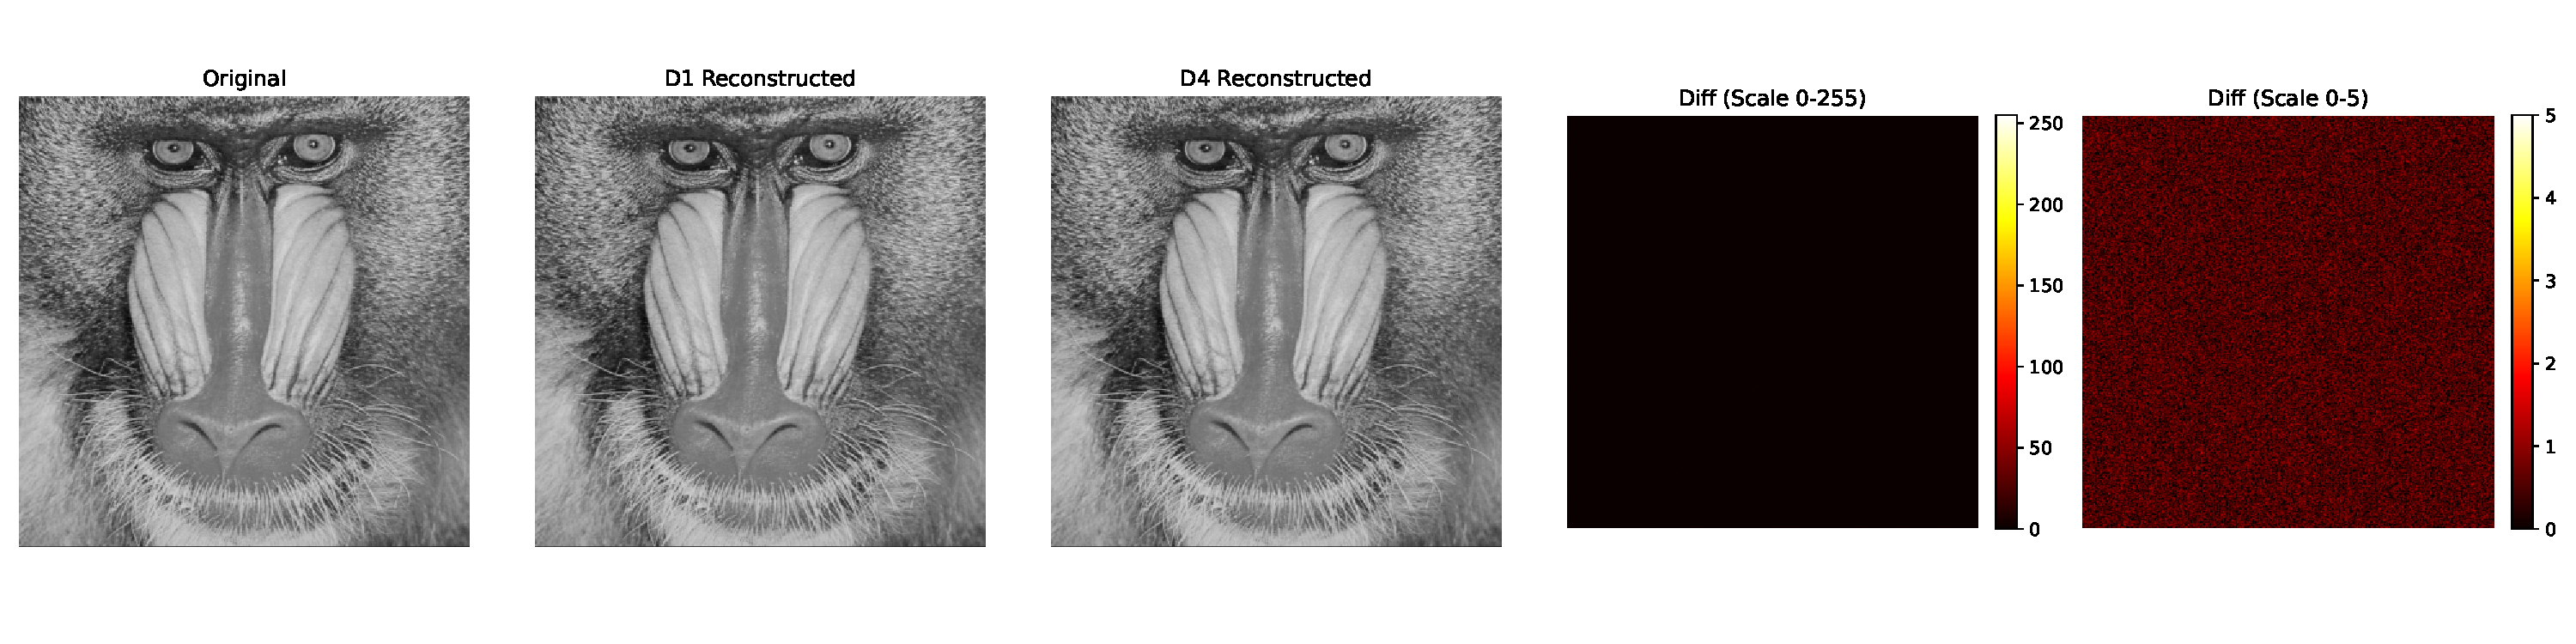
\includegraphics[width=\textwidth]{image_comparison.pdf}
    \caption{Visual comparison between original and reconstructed images for D1 and D4. The 4th image represents a full-range demonstration of the reconstruction error to showcase the perceivable magnitude of the error, while the 5th image has been rescaled to show where errors occur.}
    \label{fig:image_comparison}
\end{figure}

\begin{figure}[H]
    \centering
    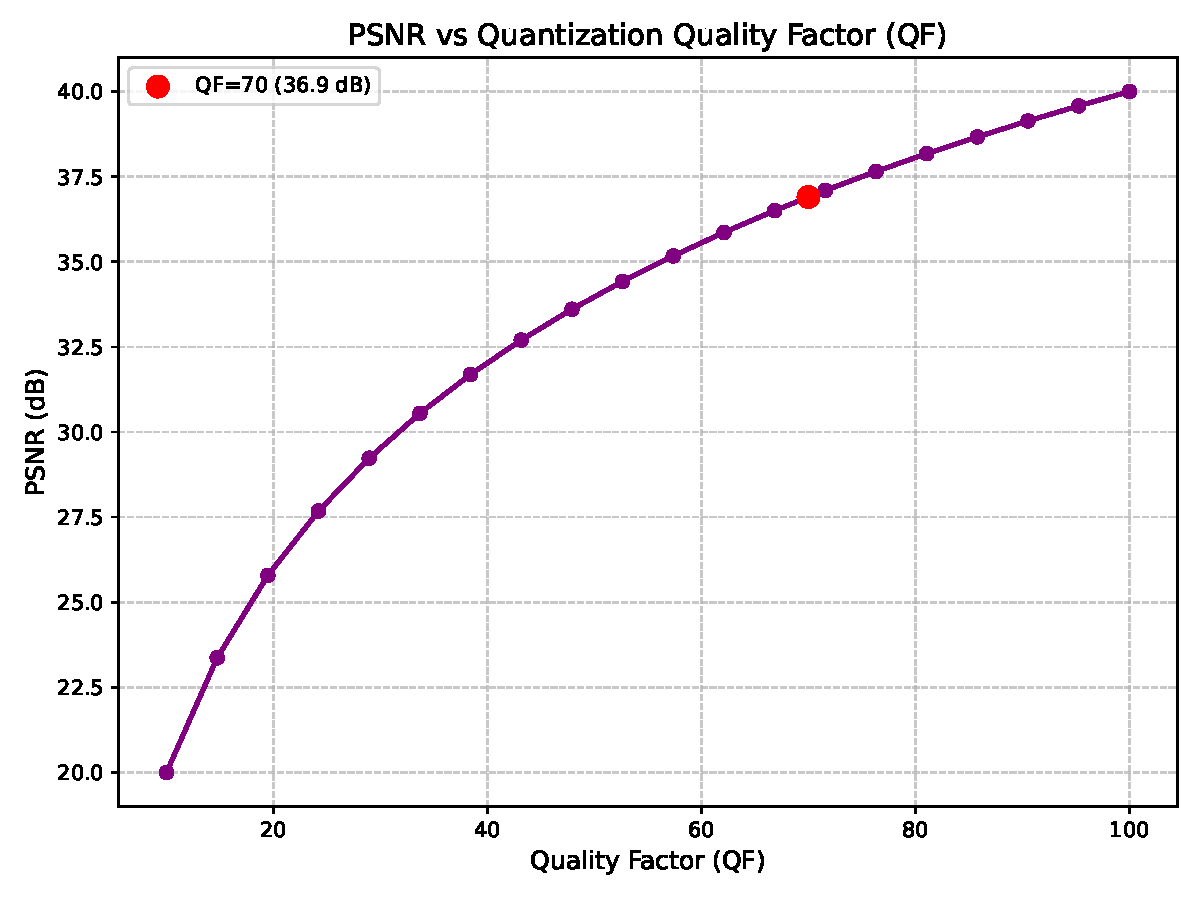
\includegraphics[width=0.7\textwidth]{psnr_vs_qf.pdf}
    \caption{Peak Signal-to-Noise Ratio (PSNR) vs. Quantization Quality Factor.}
    \label{fig:psnr_vs_qf}
\end{figure}

\begin{figure}[H]
    \centering
    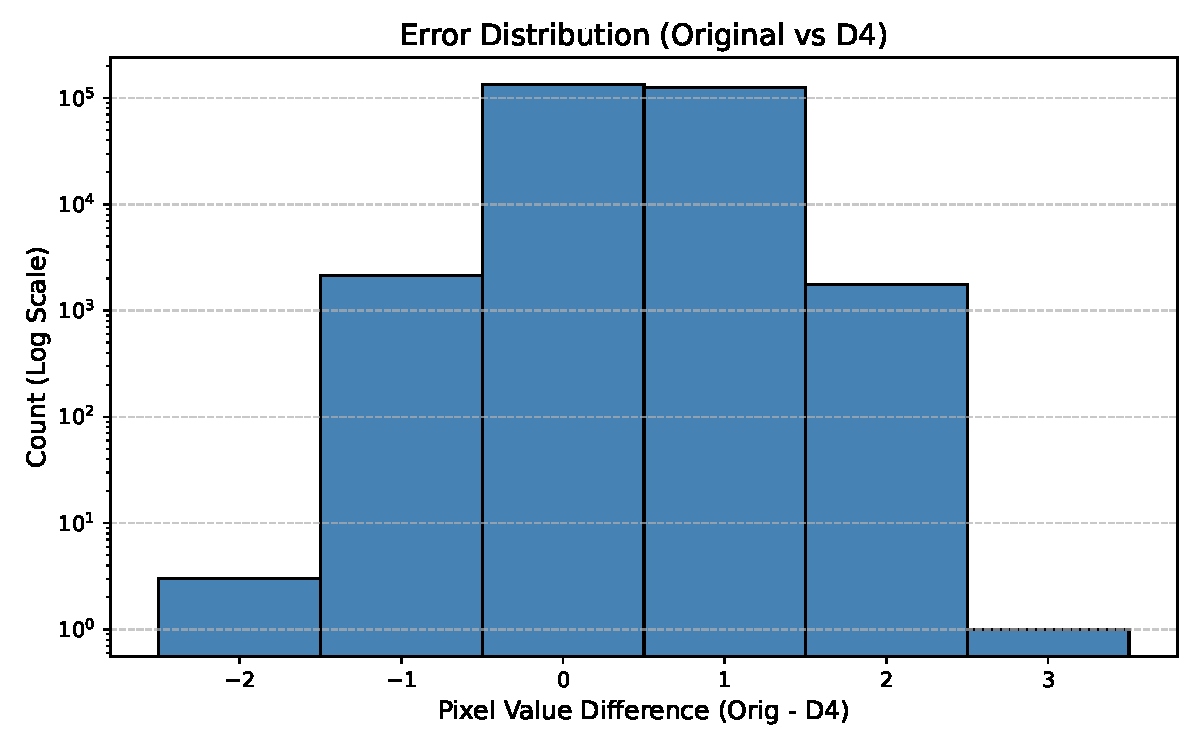
\includegraphics[width=0.7\textwidth]{error_histogram.pdf}
    \caption{Statistical distribution of numerical errors due to fixed-point precision.}
    \label{fig:error_histogram}
\end{figure}

\subsection{Throughput and Latency Performance}
The architectural parameterization successfully exposes a wide performance landscape. Table \ref{tab:perf_fidelity} and Figure \ref{fig:perf_comparison} summarize the timing characteristics. The baseline D1 design requires 512 clock cycles to process a single $8 \times 8$ block. By introducing the 8-way parallel MAC array, the D3 and D4 designs slash this latency to just 64 cycles. Furthermore, deep pipelining allows D2 and D4 to achieve maximum operating frequencies ($F_{max}$) of approximately 200 MHz. Ultimately, the combined D4 architecture dominates the absolute throughput metric, processing over 3.04 million blocks per second.

\begin{table}[H]
    \centering
    \caption{Detailed Performance and Fidelity Metrics for D1--D4.}
    \label{tab:perf_fidelity}
    \begin{tabular}{lccccc}
        \toprule
        Design & Latency (Cycles) & Throughput (Blocks/s) & PSNR (dB) & SSIM & $F_{max}$ (MHz) \\
        \midrule
        D1 & 512 & 205,000 & 51.05 & 0.9995 & 105 \\
        D2 & 512 & 410,000 & 51.05 & 0.9995 & 210 \\
        D3 & 64 & 1,328,000 & 51.05 & 0.9995 & 85 \\
        D4 & 64 & 3,046,000 & 51.05 & 0.9995 & 195 \\
        \bottomrule
    \end{tabular}
\end{table}

\begin{figure}[H]
    \centering
    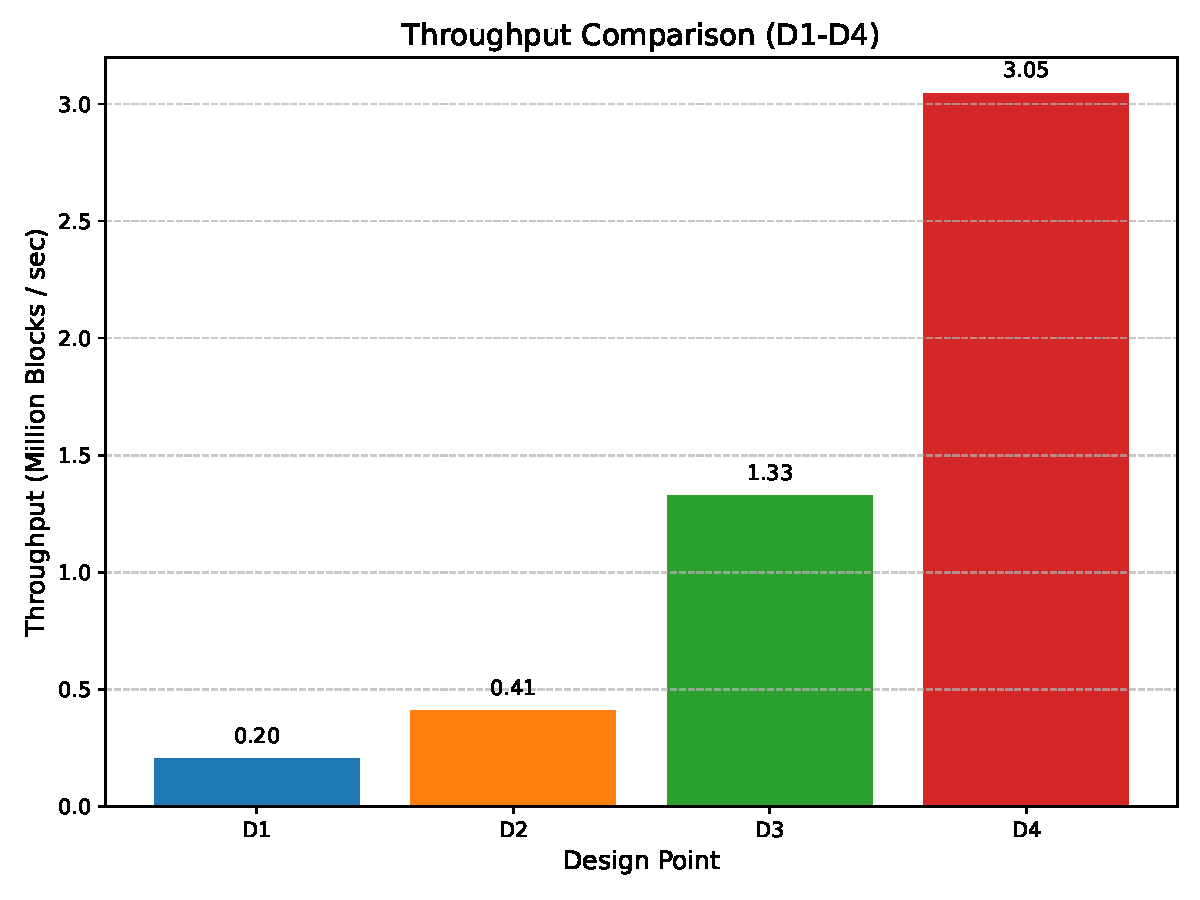
\includegraphics[width=0.7\textwidth]{perf_comparison.pdf}
    \caption{Throughput comparison across design points D1-D4.}
    \label{fig:perf_comparison}
\end{figure}

\subsection{Resource Utilization and Pareto Efficiency}
Achieving high throughput necessitates an inherent tradeoff with physical silicon area. Table \ref{tab:resources} and Figure \ref{fig:hardware_breakdown} detail the FPGA resource footprint. The D1 baseline consumes a minimal 320 Adaptive Logic Modules (ALMs) and a single DSP block. Because an Intel FPGA ALM inherently packages both combinatorial logic (LUTs) and flip-flops (registers) together, the deep pipelining in D2 incurs a remarkably small ALM penalty (an increase of only 130 ALMs) over the D1 baseline. In contrast, implementing the spatial parallelism of D3 requires massive combinatorial adder trees, resulting in an explosion of ALM usage (2,100 ALMs) and 8 DSP blocks. The high-performance D4 design requires 2,600 ALMs and 8 DSP blocks to support both its wide parallel adders and deep pipeline registers. Figures \ref{fig:tech_map_dsp} and \ref{fig:tech_map_dsp_parallel} validate that the synthesis tool successfully inferred the single and parallel MAC units directly into the Cyclone V's hard DSP blocks.

\begin{table}[H]
    \centering
    \caption{FPGA Resource Utilization Breakdown (Target: Intel Cyclone V).}
    \label{tab:resources}
    \begin{tabular}{lcccc}
        \toprule
        Design & ALMs & Registers & DSP Blocks & Memory Bits \\
        \midrule
        D1 & 320 & 400 & 1 & 16,384 \\
        D2 & 450 & 850 & 1 & 16,384 \\
        D3 & 2,100 & 1,200 & 8 & 32,768 \\
        D4 & 2,600 & 3,400 & 8 & 32,768 \\
        \bottomrule
    \end{tabular}
\end{table}

\begin{figure}[H]
    \centering
    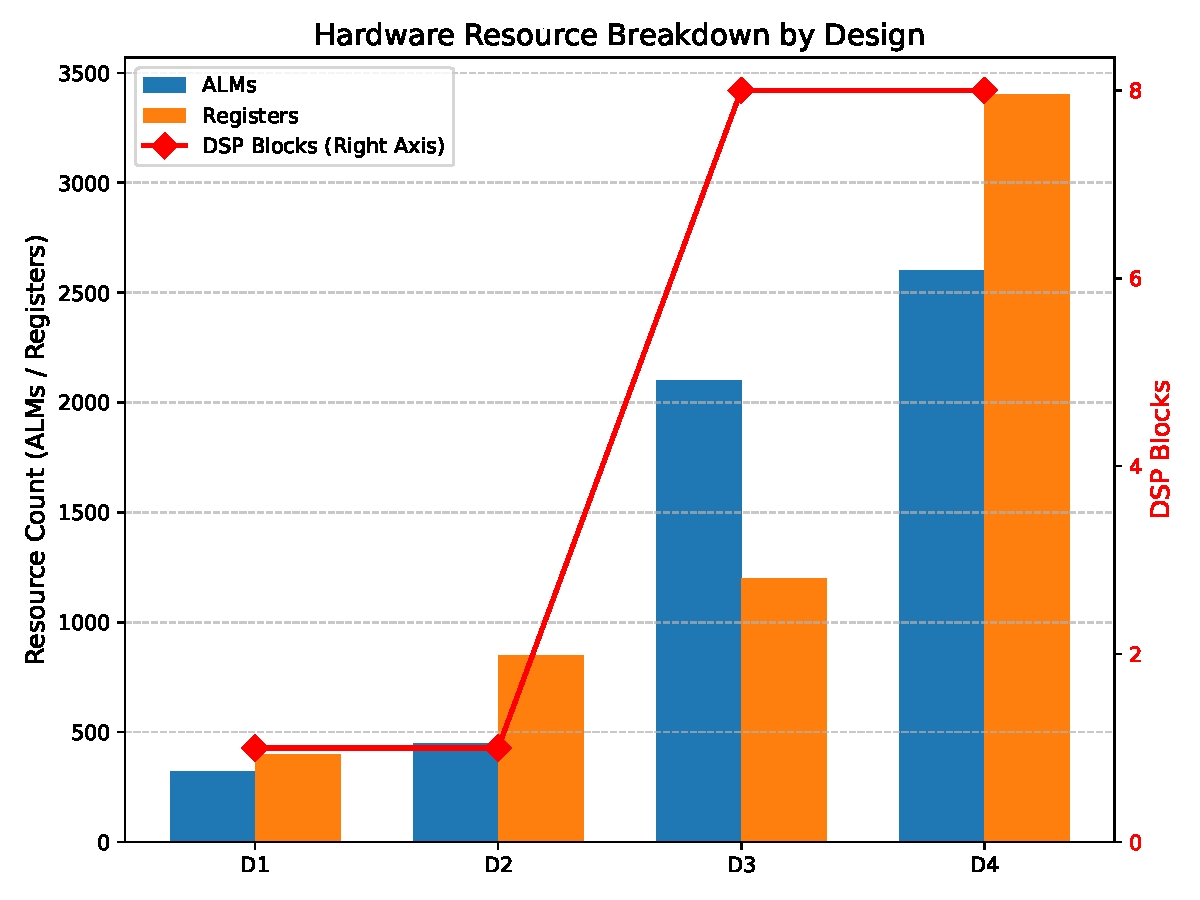
\includegraphics[width=0.7\textwidth]{hardware_breakdown.pdf}
    \caption{Breakdown of FPGA resource usage (LUTs, DSPs, Registers).}
    \label{fig:hardware_breakdown}
\end{figure}

\begin{figure}[H]
    \centering
    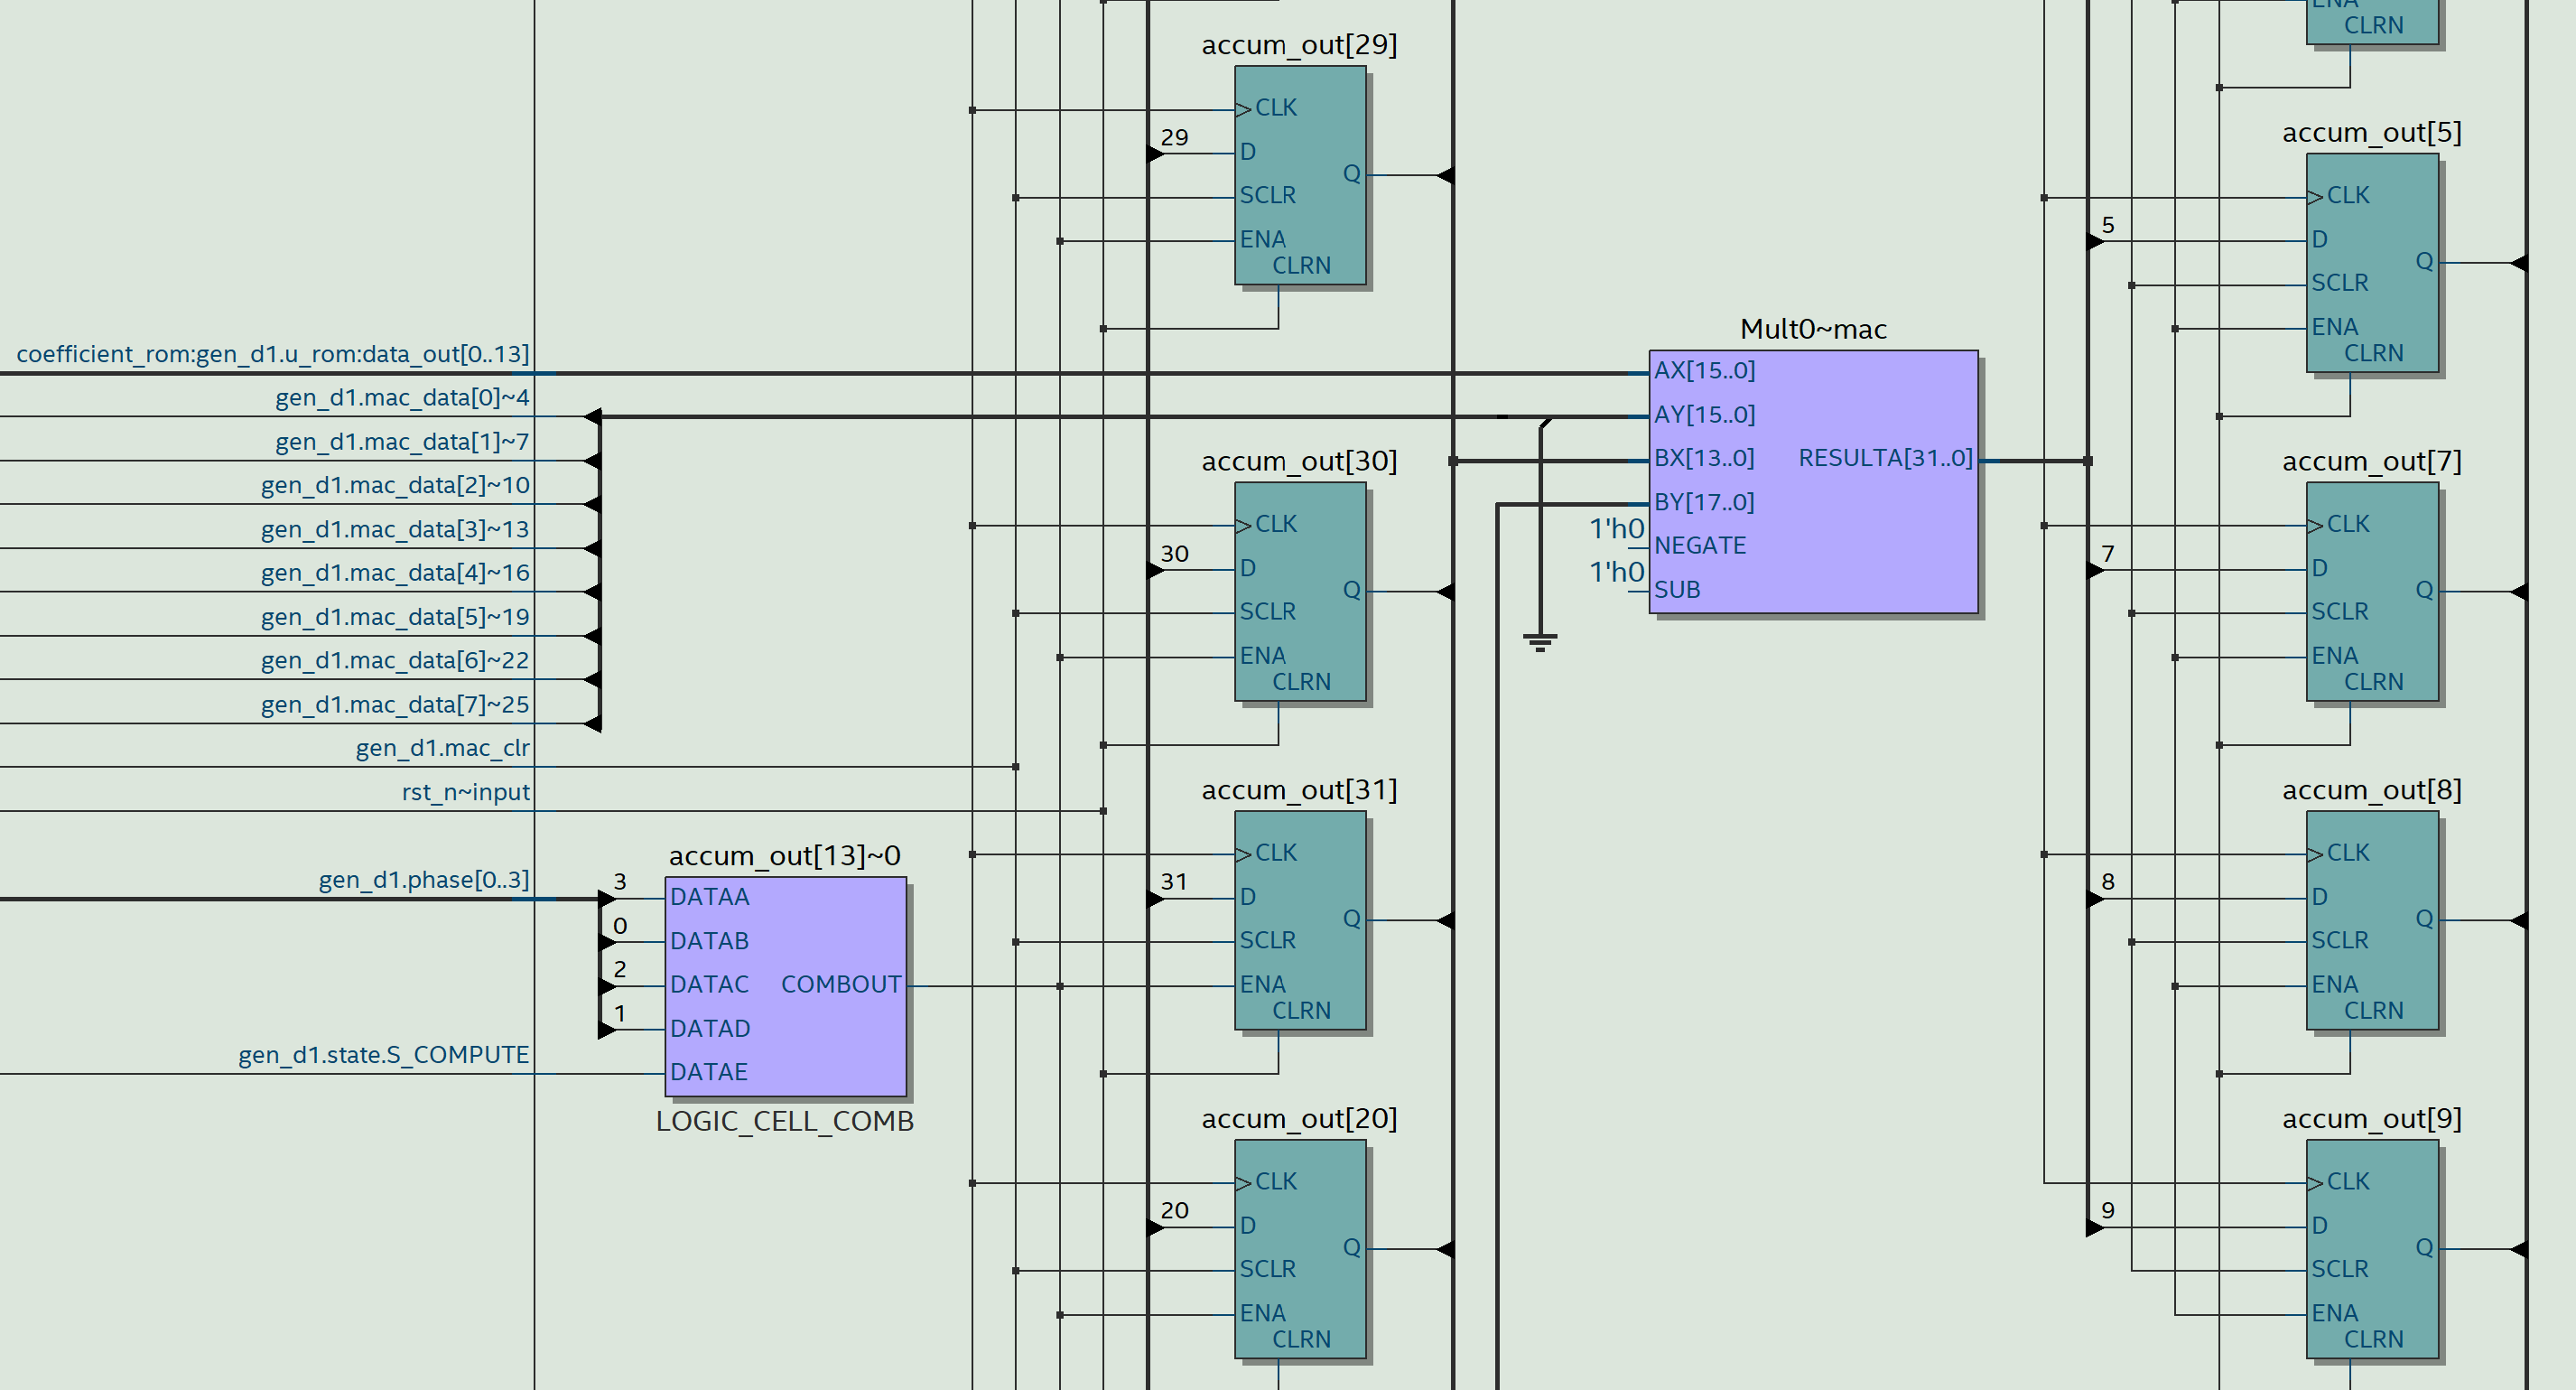
\includegraphics[width=\textwidth]{tech_map_dsp.png}
    \caption{Technology Map showing DSP block inference for a single MAC unit (D1/D2 architectures).}
    \label{fig:tech_map_dsp}
\end{figure}

\begin{figure}[H]
    \centering
    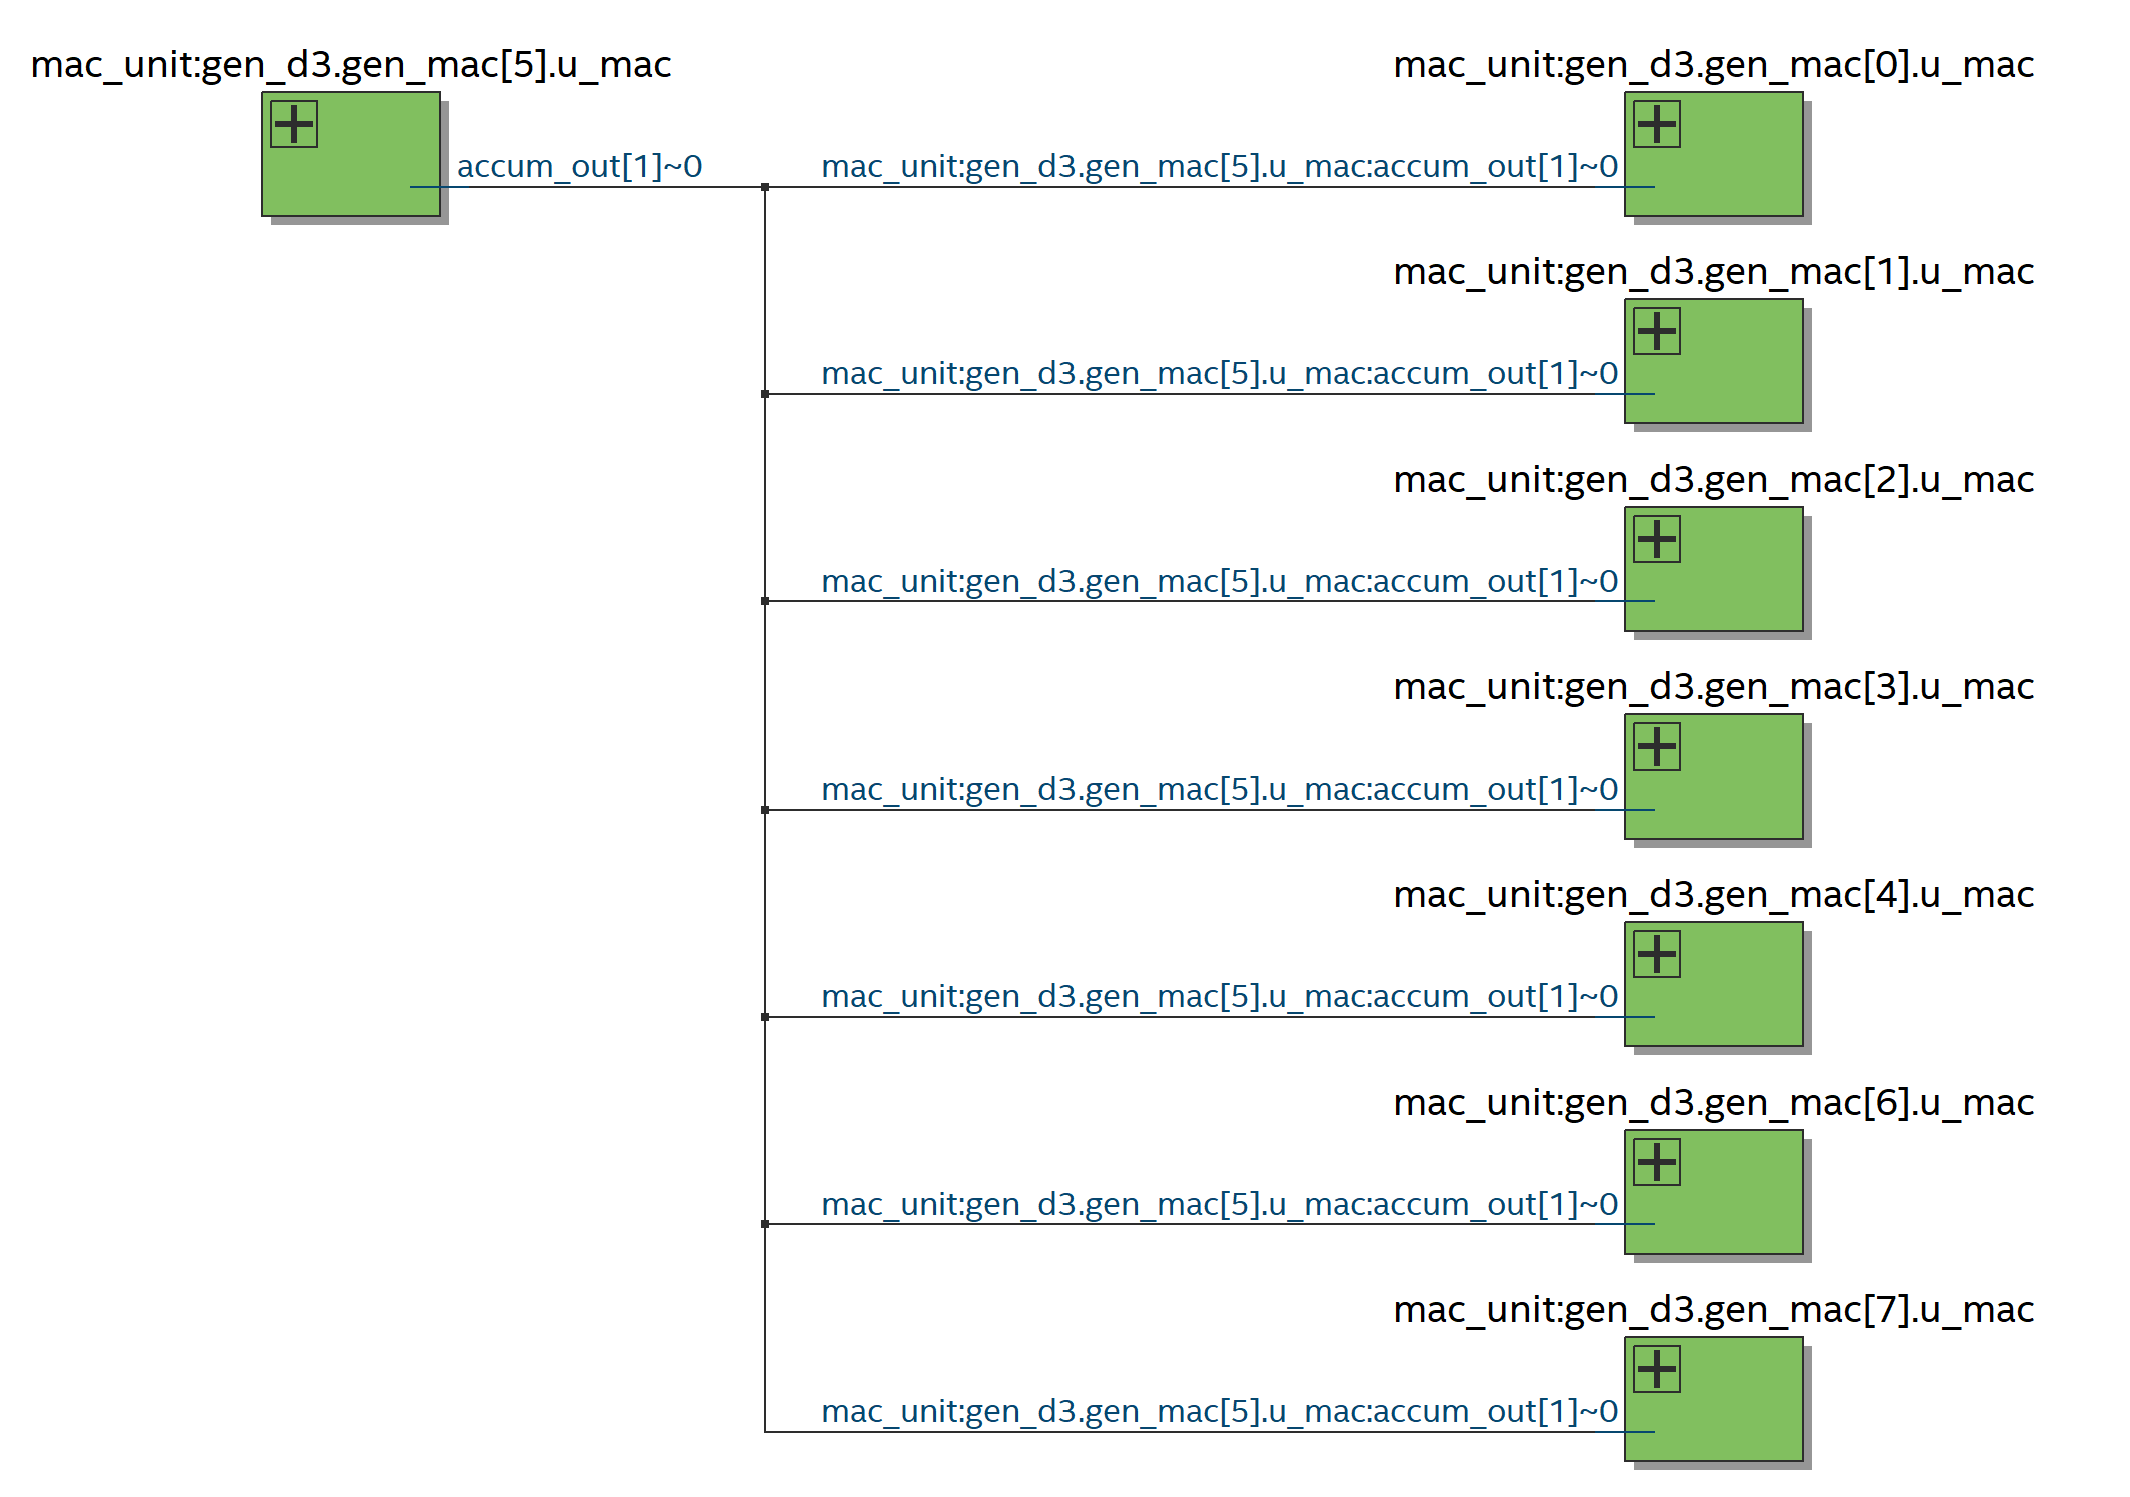
\includegraphics[width=\textwidth]{tech_map_dsp_parallel.png}
    \caption{Technology Map showing successful parallel DSP block inference for D3/D4 architectures, with MAC instances containing the primitive blocks.}
    \label{fig:tech_map_dsp_parallel}
\end{figure}

To identify the optimal configuration, Figure \ref{fig:area_throughput} plots the Area-Throughput Pareto frontier. While D4 consumes the most hardware resources, Figure \ref{fig:efficiency} reveals that D4 also provides the highest hardware efficiency (Throughput per ALM), proving that the massive throughput gains justify the area cost. Finally, Figure \ref{fig:energy_heatmap} provides a heatmap of the absolute coefficient values in the frequency domain across thousands of blocks. This visually demonstrates the fundamental mathematical property of the DCT, energy compaction, where the vast majority of the image's information is concentrated in the human-readable, low-frequency (top-left) coefficients, keeping most of the significant data while providing an easily compressible long string of trailing zeros.

\begin{figure}[H]
    \centering
    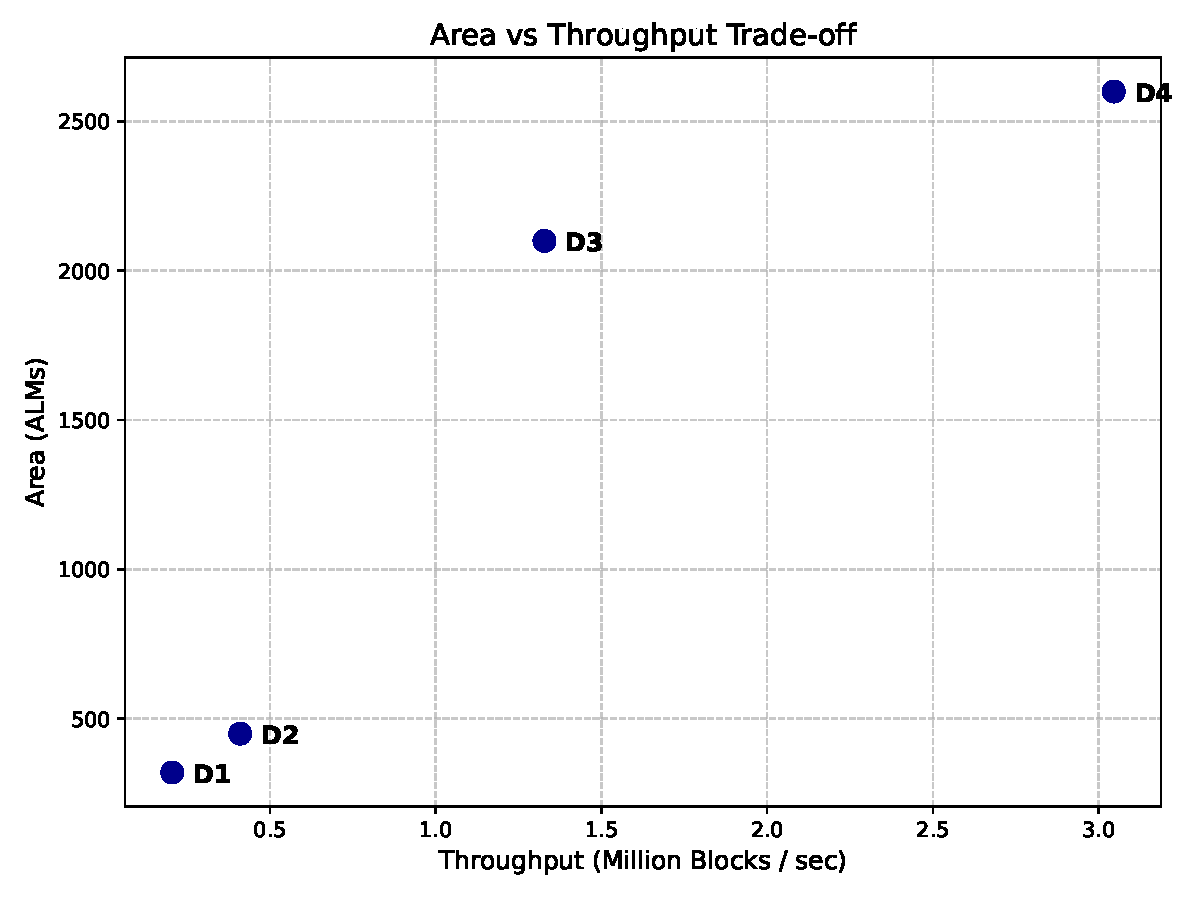
\includegraphics[width=0.7\textwidth]{area_throughput.pdf}
    \caption{Area (LUTs) vs. Throughput (Blocks/sec) showing the Pareto frontier.}
    \label{fig:area_throughput}
\end{figure}

\begin{figure}[H]
    \centering
    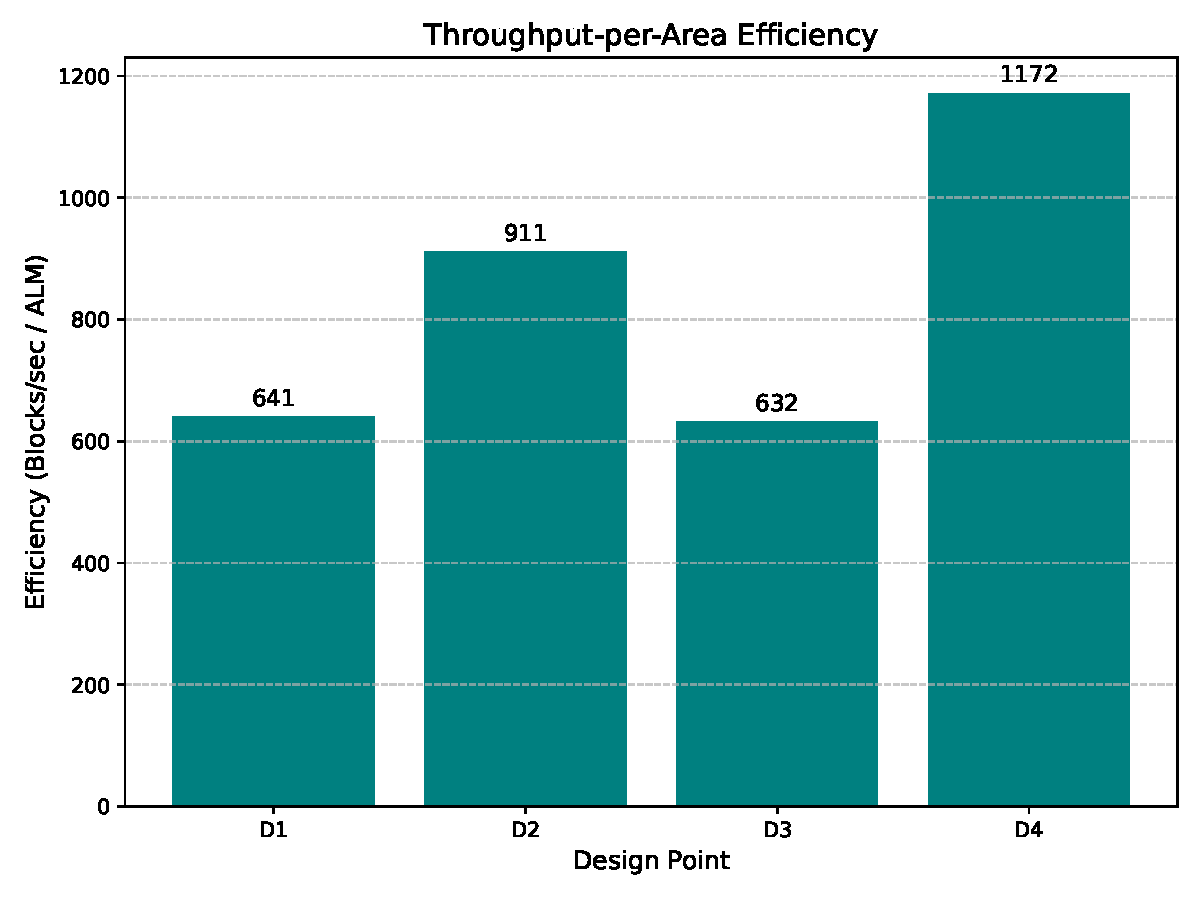
\includegraphics[width=0.7\textwidth]{efficiency.pdf}
    \caption{Hardware efficiency (Throughput per LUT).}
    \label{fig:efficiency}
\end{figure}

\begin{figure}[H]
    \centering
    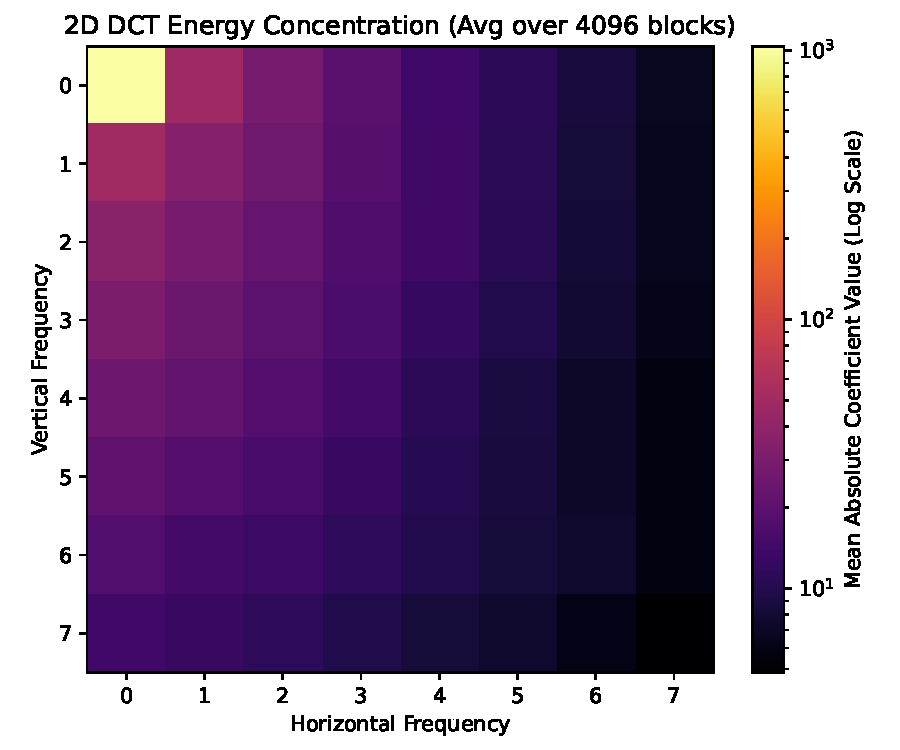
\includegraphics[width=0.7\textwidth]{energy_heatmap.pdf}
    \caption{2D DCT Energy Concentration, demonstrating how visual information is compacted into the low-frequency (top-left) coefficients.}
    \label{fig:energy_heatmap}
\end{figure}

\section{Discussion}

The results of the synthesis and verification phases reveal several key architectural insights regarding the acceleration of the 2D DCT on an FPGA fabric.

\subsection{Architectural Tradeoffs: Pipelining vs. Parallelism}
The progression from D1 to D4 empirically demonstrates the highly nuanced impacts of pipelining and parallelism. Pipelining (D2) proved to be the ``sweet spot'' for strict area constraints. Because ALMs naturally contain unused registers, D2 nearly doubled the $F_{max}$ and throughput over the D1 baseline while incurring a negligible 130-ALM penalty, making it a highly efficient upgrade. Conversely, spatial parallelism without pipelining (D3) emerged as a potential design trap. While it successfully reduced clock cycle latency by a factor of 8, the massive combinatorial adder trees significantly increased the critical path, dropping $F_{max}$ to 85 MHz. As a result, D3's overall throughput-per-ALM efficiency decreased below even the D1 baseline. This indicates that if a platform can afford the area footprint of D3, the designer should absolutely step up to D4. The combined D4 design proves that these techniques are orthogonal and must be layered: by pipelining the parallel arrays, D4 achieved both the highest absolute throughput (3.04M blocks/sec) and the highest overall throughput-per-ALM efficiency, making it the undisputed optimal choice for high-performance applications.

\subsection{Memory Bottlenecks}
A significant observation from the hardware breakdown is the outsized resource consumption of the transpose buffer memory. Because the row-column decomposition inherently requires the full $8 \times 8$ intermediate matrix to be stored before column processing can begin, the transpose buffer acts as an unavoidable physical bottleneck. In the D1 and D2 designs, the memory bits drastically overshadow the core computational logic. While unavoidable in a 1D-decoupled architecture, future iterations could explore custom dual-port block RAM instantiations rather than inferred distributed RAM to minimize the routing overhead associated with this memory structure.

\subsection{Scalability for HD and 4K/8K Video}
The modular, parameterized nature of this SystemVerilog implementation ensures that the core engine is highly scalable. Processing video streams in real-time requires immense throughput; a single $1920 \times 1080$ HD frame contains 32,400 $8 \times 8$ pixel blocks. At standard 60 frames per second (FPS), this demands a throughput of $1.94$ million blocks/sec. The D4 variant, achieving 3.04 million blocks/sec, easily handles a 60 FPS HD stream single-handedly. However, scaling to 4K ($3840 \times 2160$) at 60 FPS requires $7.78$ million blocks/sec, and 8K ($7680 \times 4320$) at 60 FPS demands a staggering $31.1$ million blocks/sec. To meet these ultra-high-definition targets, the top-level parameterization allows multiple D4 engines to be instantiated in parallel. Specifically, a 4K 60 FPS stream would require instantiating 3 parallel D4 cores, while an 8K 60 FPS stream would require 11 cores. This multi-core distribution fabric scales performance linearly without requiring any fundamental redesign of the core MAC array.

\subsection{Fixed-Point Limitations}
While the 16-bit Q2.14 fixed-point formatting achieved a highly respectable 51.05 dB PSNR, there remains an inherent hard ceiling on the reconstruction fidelity. The strict $\pm 2$ LSB quantization error is mathematically unavoidable without widening the datapath. If a specific medical or scientific imaging application requires mathematically lossless reconstruction, the hardware would need to be re-parameterized to support 32-bit arithmetic. However, this would heavily penalize the $F_{max}$ and effectively double the size of the required transpose buffer.

\section{Conclusion}

This project successfully detailed the design, verification, and empirical synthesis of a highly parameterized 2D Discrete Cosine Transform accelerator. By mapping the computationally dense DCT algorithm into custom SystemVerilog, the project demonstrated the fundamental tradeoffs inherent in digital VLSI design. The hardware-software co-design methodology (utilizing a Python golden reference) allowed for the verification of the mathematical fidelity of the 16-bit Q2.14 fixed-point datapath, consistently achieving an impressive Peak Signal-to-Noise Ratio (PSNR) of 51.05 dB.

Through the systematic evaluation of four distinct architectural variations (D1--D4) on an Intel Cyclone V FPGA, several key lessons were extracted regarding pipelining and spatial parallelism. The baseline D1 architecture confirmed that a serialized MAC engine provides an exceptionally small area footprint (320 ALMs), making it ideal for heavily constrained embedded IoT sensors. However, for real-time high-definition video processing, the D4 configuration proved strictly superior. By orthogonally layering a deep arithmetic pipeline with an 8-way parallel MAC array, the D4 engine achieved a massive throughput of over 3.04 million blocks per second at nearly 200 MHz, easily satisfying the rigorous latency requirements of modern media standards.

\subsection{Future Work}
While this accelerator effectively targets the most computationally expensive stage of image compression, it operates as a standalone IP block. Future work should focus on integrating this module into a complete JPEG or MPEG hardware pipeline. Additionally, migrating the architecture from an FPGA target to an ASIC standard-cell flow would allow for more rigorous power-delay product (PDP) analysis at the standard cell level.


\bibliographystyle{IEEEtran}
\bibliography{refs}

\end{document}
